%%%%%%%%%%%%%%%%%%%%%%%%%%%%%%%%%%%%%%%%
\chapter{Fundamento teórico}
%%%%%%%%%%%%%%%%%%%%%%%%%%%%%%%%%%%%%%%%

%%%%%%%%%%%%%%%%%%%%%%%%%%%%%%%%%%%%%%%%
\section{Polinizadores y su monitoreo}

Los polinizadores son esenciales para la reproducción de plantas y el mantenimiento de la biodiversidad global. Se estima que aproximadamente el 87\% de las plantas con flores y el 75\% de los cultivos agrícolas dependen de la polinización para su reproducción \parencite{ghosh2025pollinator}. Este servicio ecológico es crucial para los ecosistemas naturales y también
la seguridad alimentaria humana, sin embargo, su declive, debido a la destrucción del hábitat, el cambio climático y la contaminación, representa una amenaza directa para la seguridad alimentaria y la biodiversidad global. Este problema ha escalado en importancia en la última década, haciendo urgente la implementación de métodos más eficaces y precisos para su monitoreo \parencite{hellwig2024pollinator}.

Tradicionalmente, los métodos de monitoreo de polinizadores han consistido en observación directa y recolección de muestras, los cuales dependen en gran medida de la experiencia del observador y del tiempo disponible para la recolección de datos. Aunque son efectivos, estos métodos tienen limitaciones significativas: son propensos a errores humanos,
especialmente cuando se trata de especies morfológicamente similares; dependen de expertos, lo que reduce la consistencia y calidad de los datos obtenidos; y son intensivos en trabajo, lo que limita la frecuencia y extensión de los monitoreos \parencite{batz2023forecasting}.

En la actualidad, los avances en aprendizaje profundo \textit{(Deep Learning)} ofrecen soluciones innovadoras para superar estas limitaciones ya que, muestran una gran precisión y eficiencia en la detección automatizada de polinizadores a partir de imágenes aéreas, superando a los métodos tradicionales en términos de rapidez y exactitud. Este enfoque permite automatizar la clasificación de polinizadores, reducir la dependencia de expertos y minimizar los errores humanos, mejorando la fiabilidad de los datos \parencite{wang2025insectreview}.

Además, la integración de tecnologías como drones con modelos de aprendizaje
profundo facilita el monitoreo no invasivo a gran escala, lo cual mejora la calidad y frecuencia del monitoreo y permite la recolección de datos en diversas condiciones y en lugares de difícil acceso, sin interferir en el comportamiento de los polinizadores \parencite{kim2025drone}.

No obstante, el monitoreo automatizado en condiciones reales de campo introduce desafíos técnicos que pueden degradar el desempeño de los modelos de visión por computador. Entre los principales se encuentran la variabilidad de iluminación natural, los fondos complejos que dificultan separar el insecto del entorno, la oclusión parcial por vegetación y el desenfoque por movimiento debido a la rapidez de los polinizadores. 

Adicionalmente, el tamaño reducido de muchas especies, la variación de escala y punto de vista en capturas aéreas o con cámaras fijas, y la alta similitud visual entre taxones incrementan la probabilidad de confusión en la clasificación. A ello se suman dificultades propias de los datos ecológicos, como el desbalance de clases, la disponibilidad limitada de imágenes etiquetadas y el \textit{domain shift}, que ocurre cuando un modelo entrenado en un escenario pierde capacidad de generalización al aplicarse en ambientes, estaciones o configuraciones de captura distintas \parencite{stefan2025successes}.

En cuanto a la conservación de los polinizadores, el uso de modelos de aprendizaje profundo en combinación con programas de monitoreo a gran escala y la integración de la ciencia se presentan como herramientas clave para comprender mejor las dinámicas de las poblaciones de polinizadores y mitigar su declive \parencite{hellwig2024pollinator}. 

%%%%%%%%%%%%%%%%%%%%%%%%%%%%%%%%%%%%%%%%
\section{Fundamentos del aprendizaje profundo }

El aprendizaje profundo es una subdisciplina del aprendizaje automático que se centra en modelar datos a través de múltiples capas de neuronas, utilizando estructuras complejas y transformaciones no lineales \parencite{bhargavi2020survey}. Este enfoque está inspirado en el funcionamiento del cerebro humano, permitiendo procesar información a través de niveles jerárquicos para entender representaciones y características a partir de datos sin procesar.

A través de esta jerarquización, el aprendizaje profundo ha sido capaz de abordar problemas de alta complejidad, como el reconocimiento de imágenes, el procesamiento del lenguaje natural y la predicción de patrones en grandes volúmenes de datos. Una de las principales características del aprendizaje profundo es su uso de modelos de redes neuronales profundas, las cuales sirven como puente para representar grandes cantidades de datos y aprender relaciones complejas dentro de ellos \parencite{sharma2020deepintro}.

El aprendizaje profundo ha mostrado un rendimiento destacado en varias áreas, lo que demuestra su versatilidad y eficacia. En visión por computadora, se ha utilizado para tareas como la clasificación de imágenes y la detección de objetos, mientras que en el reconocimiento de voz ha facilitado el procesamiento y reconocimiento de patrones vocales \parencite{zulkernine2020tutorial}, permitiendo avances en sistemas de asistencia virtual. En el ámbito de la biología, se utiliza para tareas como la identificación de especies, el monitoreo ambiental y el modelado ecológico, contribuyendo a la conservación de la biodiversidad y la mejora de la sostenibilidad ambiental \parencite{borowiec2022deep}.

\subsection{Diferencias entre aprendizaje automático tradicional y aprendizaje profundo}

El aprendizaje automático tradicional suele depender de ingeniería de características, es decir, del diseño manual de descriptores antes de entrenar el modelo. Esto exige conocimiento del dominio y puede limitar el desempeño cuando la variabilidad visual es alta \parencite{rajasree2025feature,chen2024tradeoff}.

El aprendizaje profundo, en cambio, se apoya en aprendizaje de representaciones, donde redes neuronales aprenden automáticamente características jerárquicas a partir de datos sin procesar. Este enfoque ha mostrado alta eficacia en reconocimiento, detección y segmentación de objetos \parencite{khastavaneh2020representation}.

Los métodos tradicionales pueden ser competitivos con menos datos cuando las características son informativas, mientras que el aprendizaje profundo suele requerir más datos etiquetados, aunque su rendimiento puede sostenerse en escenarios de datos reducidos mediante configuraciones adecuadas \parencite{edwin2022smallscale,rajasree2025feature}.

En términos prácticos, el aprendizaje profundo demanda mayor cómputo y memoria, por lo que se beneficia del uso de GPU y análisis de eficiencia. Además, suele presentar menor interpretabilidad directa, pese a que generalmente logra mayor desempeño en problemas visuales complejos; en sistemas con restricciones energéticas, la eficiencia de las representaciones es un factor crítico \parencite{staka2025cpugpu,chen2024tradeoff}.


%%%%%%%%%%%%%%%%%%%%%%%%%%%%%%%%%%%%%%%%
\section{Visión computacional}

La visión computacional es un campo dentro de la inteligencia artificial que permite a las máquinas interpretar y comprender el contenido visual de imágenes y videos, de manera similar a como lo haría un ser humano. En el contexto de la identificación de polinizadores, la visión computacional utiliza redes neuronales convolucionales (CNN, por sus siglas en inglés \textit{Convolutional Neural Networks}) para realizar tareas como clasificación, detección y segmentación de imágenes. 

La clasificación implica asignar una etiqueta a una imagen completa, como identificar la especie de un insecto en una fotografía. En el ámbito de la identificación de polinizadores, la clasificación es crucial para distinguir entre diferentes especies de insectos. Un estudio reciente utilizó CNN para clasificar insectos en imágenes de alta resolución capturadas por trampas de cámara, logrando una precisión media (mAP, por sus siglas en inglés \textit{Mean Average Precision}) del 54,23\% en la clasificación a nivel de orden \parencite{sadoun2024camera}. 

En cuanto a la detección, esta implica identificar y localizar objetos específicos dentro de una imagen. En el caso de los polinizadores, la detección se refiere a localizar la presencia de abejas en imágenes de un campo o una colmena. En esta línea, \parencite{sadoun2024camera} desarrollaron un estudio aplicado de monitoreo ambiental de alta resolución, en el que emplearon la red YOLOv8 para detectar insectos polinizadores en imágenes obtenidas mediante trampas de cámara macro. Sus resultados mostraron el potencial de este enfoque para recolectar datos precisos a nivel de especie.

Por su parte, la segmentación es una técnica que permite dividir una imagen en regiones significativas, como separar un polinizador del fondo \parencite{indu2023leaf}. Existen dos tipos principales de segmentación: segmentación semántica y segmentación de instancias. 

La segmentación semántica asigna una etiqueta a cada píxel de la imagen, un estudio utilizó U-Net, una arquitectura popular para la segmentación de imágenes, para segmentar imágenes de epífitas adquiridas con drones, evaluando los resultados con el índice de Jaccard y el puntaje Dice \parencite{raheesh2022ophytis}. Por otro lado, la segmentación de instancias
distingue entre diferentes objetos de la misma clase, se aplica en redes como Mask R-CNN, que ha sido utilizada para identificar automáticamente lesiones en hojas de tomate, logrando una precisión promedio del 73,00\% \parencite{kaur2024hybrid}. \\

\newcommand{\subdesc}[1]{\footnotesize \textit{#1}\par}

\begin{figure}[h]
    \centering
    \caption{Representación esquemática de tareas de visión por computador.}
    
    % --- FILA 1 ---
    \begin{subfigure}[t]{0.47\textwidth}
        \centering
        \caption{Clasificación}
        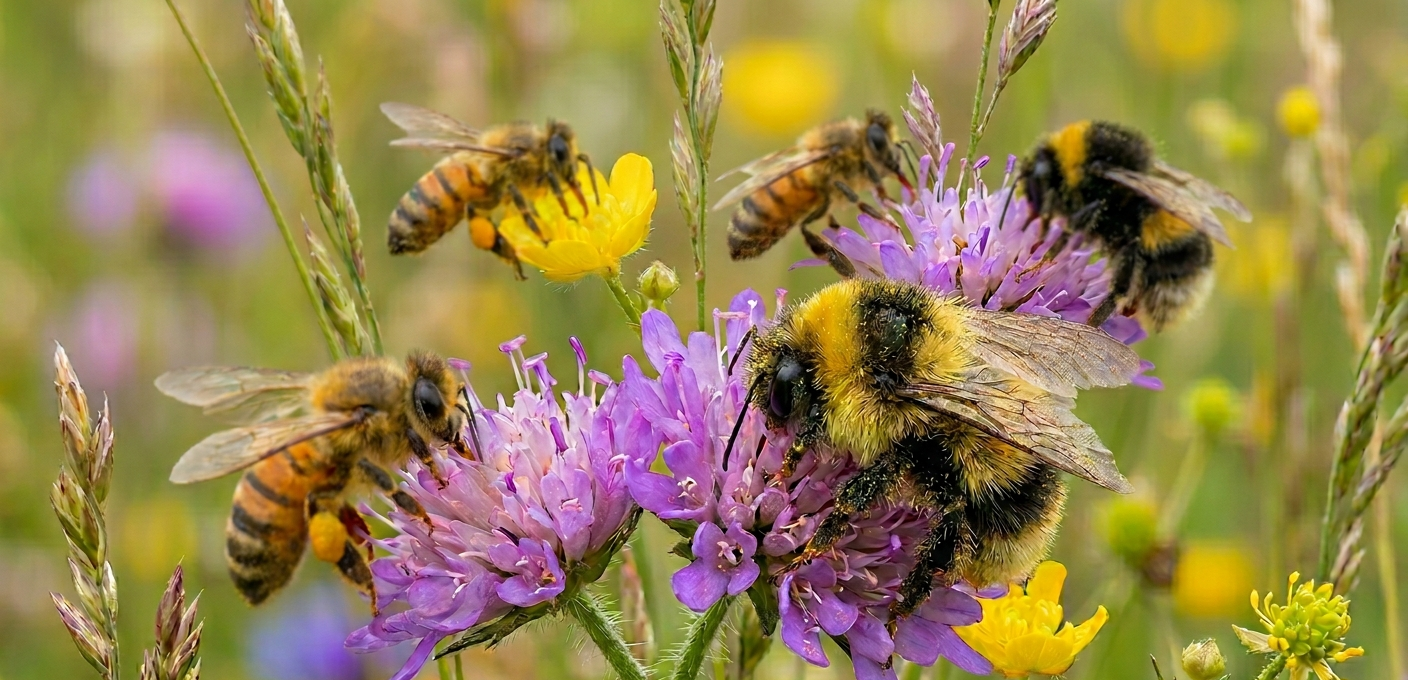
\includegraphics[width=\linewidth]{Figuras/Clasificacion_VC.png}
        \subdesc{Identificación de la clase principal en la imagen: Abeja.}
    \end{subfigure}
    \hfill
    \begin{subfigure}[t]{0.47\textwidth}
        \centering
        \caption{Detección de objetos}
        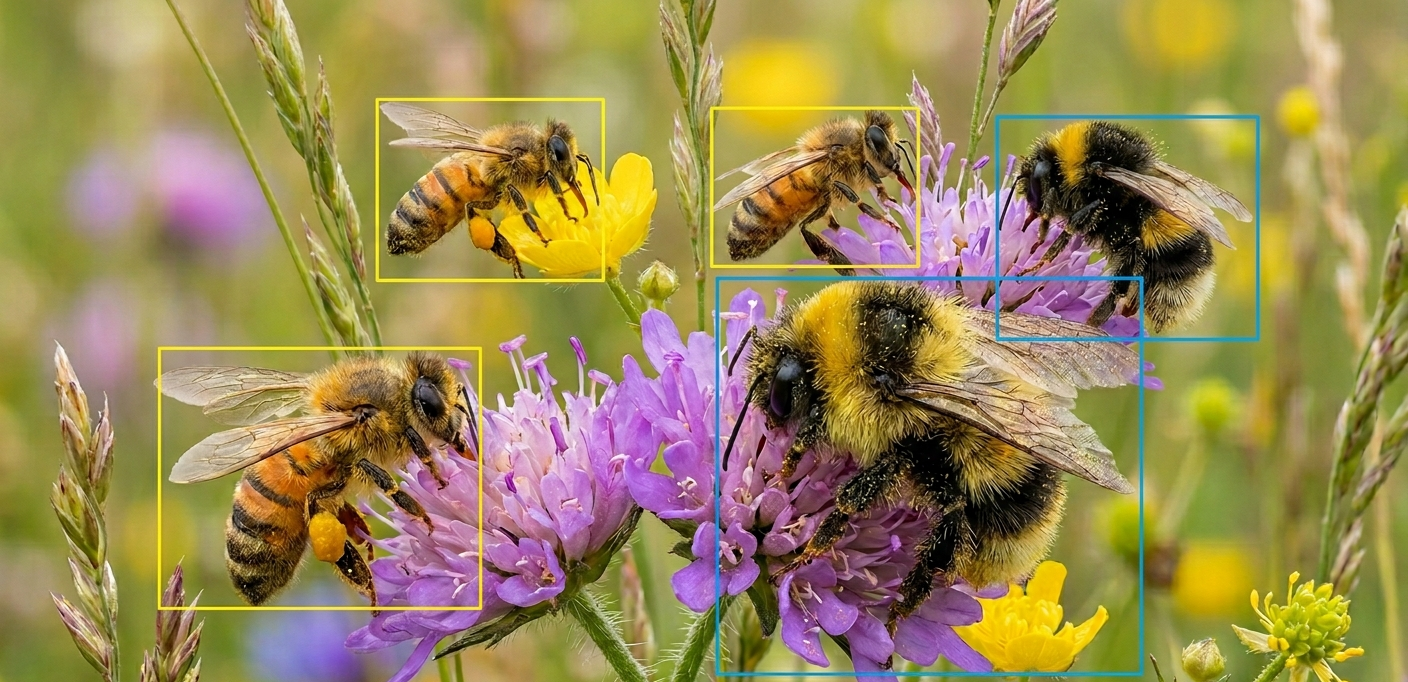
\includegraphics[width=\linewidth]{Figuras/Detección_VC.png} 
        \subdesc{Localización y clasificación de abejas y abejorros mediante cajas delimitadoras.}
    \end{subfigure}
    
    \vspace{0.6cm}
    
    % --- FILA 2 ---
    \begin{subfigure}[t]{0.47\textwidth}
        \centering
        \caption{Segmentación semántica}
        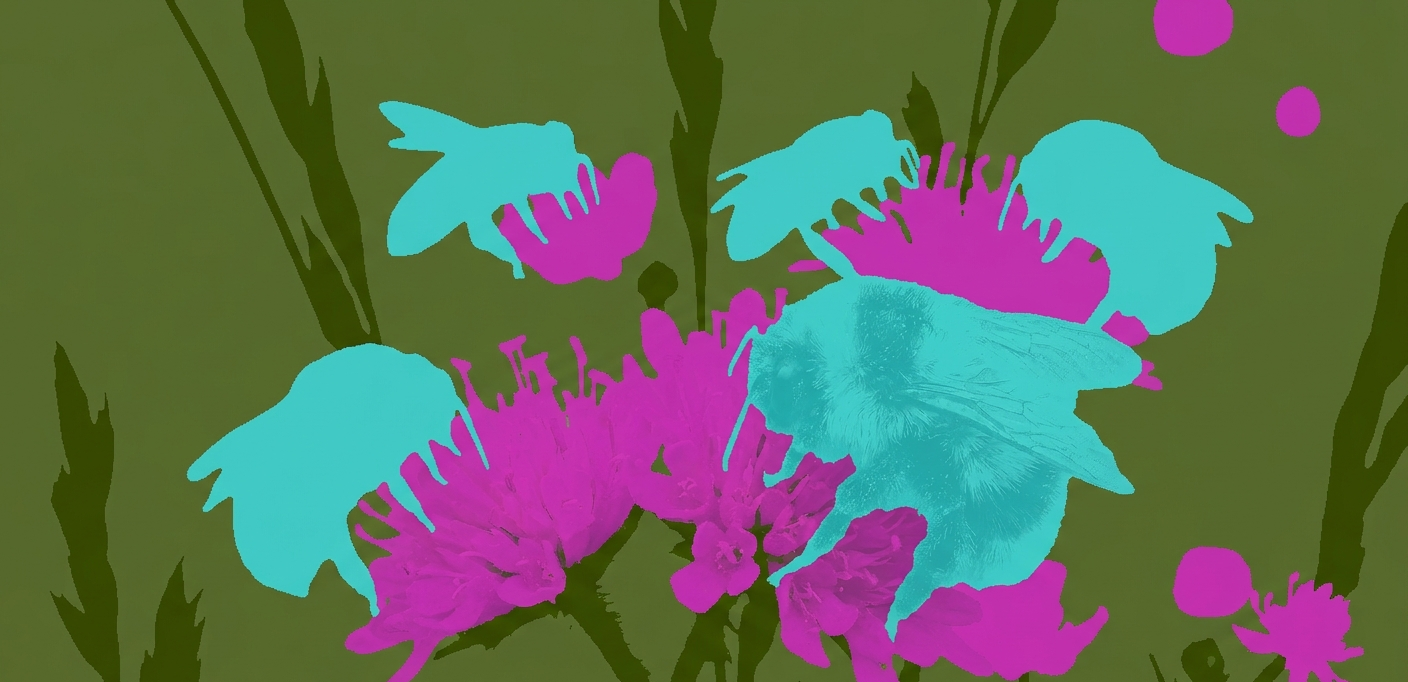
\includegraphics[width=\linewidth]{Figuras/Segmentación semántica_VC.png}
        \subdesc{Asignación de una categoría a cada píxel según la clase del objeto.}
    \end{subfigure}
    \hfill
    \begin{subfigure}[t]{0.47\textwidth}
        \centering
        \caption{Segmentación de instancia}
        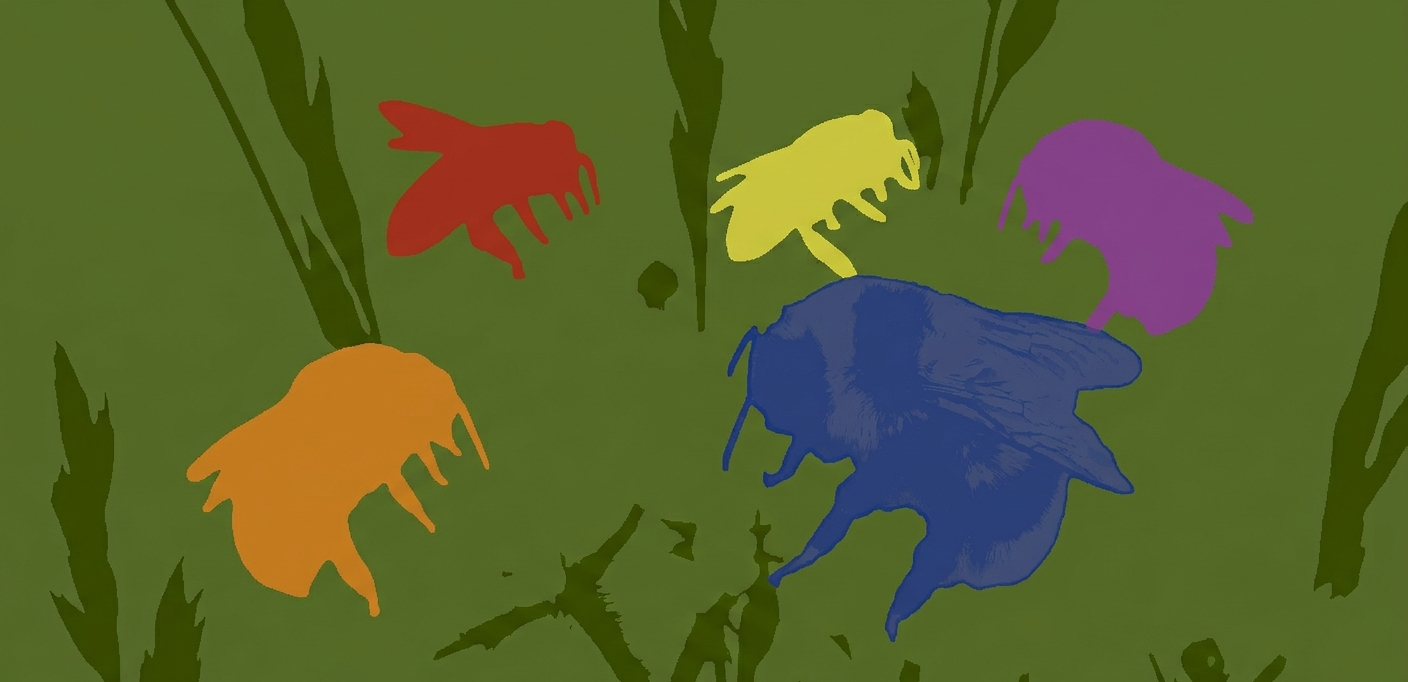
\includegraphics[width=\linewidth]{Figuras/Segmentación instancia_VC.png}
        \subdesc{Separación individual de cada polinizador como una instancia distinta.}
    \end{subfigure}


    
    \vspace{0.2cm}
    \caption*{\normalfont\normalsize\textit{Nota.} Elaboración propia.}
    
    \label{fig:tareas_vision_polinizadores}
\end{figure}

La Figura \ref{fig:tareas_vision_polinizadores} presenta una representación esquemática de las principales tareas de visión por computador aplicadas al reconocimiento de polinizadores. En clasificación, el modelo asigna una única etiqueta al objeto principal de la imagen. En detección, identifica y localiza múltiples objetos mediante cajas delimitadoras. En segmentación semántica, clasifica regiones de la imagen de acuerdo con su clase, sin distinguir individuos de una misma categoría. Finalmente, en segmentación de instancia, separa cada objeto de forma individual, incluso cuando varios pertenecen a la misma clase.

%%%%%%%%%%%%%%%%%%%%%%%%%%%%%%%%%%%%%%%%
\section{Redes Neuronales}

Las redes neuronales son sistemas computacionales inspirados en el cerebro
humano, compuestos por múltiples capas de neuronas artificiales que procesan información y aprenden a realizar tareas específicas mediante el ajuste de sus conexiones internas. Existen varias arquitecturas de redes neuronales, siendo las redes neuronales convolucionales las más utilizadas en el reconocimiento de imágenes debido a su capacidad para aprender y generalizar patrones complejos \parencite{stark2025pollinators}.

En el reconocimiento de imágenes, las técnicas de extracción de características juegan un papel crucial, ya que permiten identificar y representar elementos visuales importantes de una imagen, facilitando su clasificación y análisis \parencite{sajib2025comparative}. Los beneficios de las redes neuronales en el reconocimiento de imágenes incluyen alta precisión en tareas de clasificación, la automatización de procesos que antes requerían intervención humana, y su adaptabilidad a diferentes tipos de datos y tareas, lo que las hace muy versátiles en diversas aplicaciones.

\subsection{Arquitectura general de una red neuronal profunda}

Una red neuronal profunda se organiza en una jerarquía de capas que transforma progresivamente los datos de entrada hasta producir una salida, usualmente una predicción de clase o una estimación continua. En visión por computador, esta organización se concreta en bloques que extraen y combinan características, lo que permite construir representaciones internas cada vez más informativas para la tarea \parencite{khan2020survey}.

En este tipo de modelos, las capas iniciales aprenden representaciones de bajo nivel, como bordes, texturas y patrones simples, mientras que las capas más profundas integran dichas señales para formar representaciones de mayor nivel asociadas con formas y estructuras complejas, facilitando la discriminación de objetos o categorías visuales. Esta propiedad constituye la base del aprendizaje jerárquico de representaciones en redes profundas \parencite{zakeri2023vision,zurowietz2020feature}.

La capacidad de una red para modelar relaciones complejas depende, entre otros aspectos, de su profundidad y su ancho. Aumentar la profundidad incrementa el número de transformaciones sucesivas y favorece la construcción de representaciones más abstractas, mientras que aumentar el ancho incrementa la cantidad de unidades por capa y, con ello, la diversidad de patrones que pueden ser capturados en una misma etapa de procesamiento  \parencite{khan2020survey}.

En aplicaciones de clasificación de imágenes, es común que la arquitectura incluya capas que extraen características, mecanismos de reducción de dimensionalidad y capas finales que integran la información para producir la predicción. Esta organización permite que el modelo aprenda representaciones compactas que preservan información relevante y reduzcan redundancias, mejorando la capacidad de generalización cuando se diseña y ajusta adecuadamente \parencite{khan2020survey,chandraprakash2024spss}.

\subsubsection{Capas}

Una red neuronal profunda se estructura en capas con funciones diferenciadas dentro del proceso de propagación hacia adelante. Cada capa transforma progresivamente la representación de los datos, permitiendo que el modelo construya descripciones internas cada vez más adecuadas para la tarea de clasificación.

La capa de entrada recibe los datos en forma numérica y establece la representación inicial sobre la cual operará el modelo. Su función principal es garantizar que la información sea correctamente incorporada al sistema, sin realizar transformaciones complejas. \parencite{joselin2024healthcare}.

Las capas ocultas constituyen el núcleo del proceso de aprendizaje. A través de transformaciones sucesivas, estas capas modifican la representación de los datos, permitiendo capturar patrones, dependencias y estructuras internas. La presencia de múltiples capas favorece la construcción de representaciones jerárquicas, en las cuales la información es refinada progresivamente hasta volverse más adecuada para la decisión final. La profundidad y la anchura de la red influyen directamente en su capacidad de representación y en la complejidad de las funciones que puede aproximar. \parencite{kamho2022complexity,apicella2024hidden}.

La profundidad y el ancho de la red influyen directamente en su capacidad de representación. Una arquitectura suficientemente profunda permite modelar transformaciones complejas mediante etapas sucesivas, mientras que una anchura adecuada contribuye a la formación de regiones de decisión más flexibles en el espacio de características \parencite{chaturvedi2023activation}.

Finalmente, la capa de salida produce la respuesta final del modelo. Su estructura depende de la naturaleza de la tarea, pudiendo generar una etiqueta única, múltiples etiquetas, coordenadas espaciales o mapas estructurados. En todos los casos, esta capa sintetiza la información transformada por las capas previas y la convierte en una predicción interpretable. \parencite{liu2024binary}. \\

\begin{figure}[h]
    \centering
    \caption{Arquitectura general de una red neuronal profunda.}
    \label{fig:arquitectura_red_profunda}
    
    \begin{tikzpicture}[
        neurona/.style={circle, draw, minimum size=0.7cm},
        etiqueta/.style={align=center, font=\small},
        activacion/.style={
            draw,
            rounded corners,
            align=center,
            font=\scriptsize,
            minimum width=2.6cm,
            minimum height=0.9cm
        },
        perdida/.style={
            draw,
            rounded corners,
            align=center,
            font=\scriptsize,
            minimum width=2.8cm,
            minimum height=1cm
        }
    ]
    
    % Capa de entrada
    \node[neurona] (I1) {};
    \node[neurona, below=0.6cm of I1] (I2) {};
    \node[neurona, below=0.6cm of I2] (I3) {};
    \node[neurona, below=0.6cm of I3] (I4) {};
    \node[neurona, below=0.6cm of I4] (I5) {};
    \node[etiqueta, above=0.4cm of I1] {Capa de entrada};
    
    % Capa oculta 1
    \node[neurona, right=2cm of I1] (H11) {};
    \node[neurona, below=0.6cm of H11] (H12) {};
    \node[neurona, below=0.6cm of H12] (H13) {};
    \node[neurona, below=0.6cm of H13] (H14) {};
    \node[etiqueta, above=0.4cm of H11] {Capa oculta 1};
    
    % Capa oculta 2
    \node[neurona, right=2cm of H11] (H21) {};
    \node[neurona, below=0.6cm of H21] (H22) {};
    \node[neurona, below=0.6cm of H22] (H23) {};
    \node[neurona, below=0.6cm of H23] (H24) {};
    \node[etiqueta, above=0.4cm of H21] {Capa oculta 2};
    
    % Capa oculta 3
    \node[neurona, right=2cm of H21] (H31) {};
    \node[neurona, below=0.6cm of H31] (H32) {};
    \node[neurona, below=0.6cm of H32] (H33) {};
    \node[neurona, below=0.6cm of H33] (H34) {};
    \node[etiqueta, above=0.4cm of H31] {Capa oculta 3};
    
    % Capa de salida
    \node[neurona, right=2cm of H31] (O1) {};
    \node[neurona, below=0.6cm of O1] (O2) {};
    \node[etiqueta, above=0.4cm of O1] {Capa de salida};
    
    % Conexiones completas
    \foreach \i in {I1,I2,I3,I4,I5}
        \foreach \j in {H11,H12,H13,H14}
            \draw (\i) -- (\j);
    
    \foreach \i in {H11,H12,H13,H14}
        \foreach \j in {H21,H22,H23,H24}
            \draw (\i) -- (\j);
    
    \foreach \i in {H21,H22,H23,H24}
        \foreach \j in {H31,H32,H33,H34}
            \draw (\i) -- (\j);
    
    \foreach \i in {H31,H32,H33,H34}
        \foreach \j in {O1,O2}
            \draw (\i) -- (\j);
    
    % Punto medio de salida
    \coordinate (OutMid) at ($(O1)!0.5!(O2)$);
    
    % Caja de activación
    \node[activacion, below=2.1cm of H23] (A) {Funciones de activación\\ $\sigma(z)$};
    
    % Línea horizontal bajo capas ocultas
    \draw[thick] ($(H14.south)+(0,-0.35)$) -- ($(H34.south)+(0,-0.35)$);
    
    % Línea discontinua hacia la caja
    \draw[dashed] ($(H24.south)+(0,-0.35)$) -- ($(A.north)+(0,0.05)$);
    
    % Función de pérdida
    \node[perdida, right=2.2cm of A] (L)
    {Función de pérdida\\$\mathcal{L}(y,\hat{y})$};
    
    % Flecha vertical recta
    \coordinate (lineaRef) at ($(H24.south)+(0,-0.35)$);
    \draw[->, thick] ($(O2.south)+(0,-0.1)$) -- ($(lineaRef -| O2)$);
    
    \end{tikzpicture}
    
    \vspace{0.2cm}
    \caption*{\normalfont\normalsize\textit{Nota.} Elaboración propia.}
\end{figure}

En la Figura \ref{fig:arquitectura_red_profunda} se detalla la arquitectura general de una red neuronal profunda, en la cual la información fluye desde la entrada hacia la salida mediante transformaciones sucesivas. En cada capa oculta se aplican funciones de activación después de las transformaciones lineales, introduciendo no linealidad y permitiendo modelar relaciones complejas. En la capa de salida también se emplea una función de activación adecuada según la tarea. La función de pérdida se define sobre las salidas finales del modelo y mide la discrepancia entre las predicciones y los valores reales, generando la señal de error utilizada durante el entrenamiento.

\subsubsection{Funciones de activación y pérdida}

Las funciones de activación introducen no linealidad en las redes neuronales profundas, permitiendo modelar relaciones complejas en tareas de clasificación, detección y segmentación. En las capas ocultas, estas funciones se aplican después de cada transformación lineal, mientras que en la capa de salida se seleccionan en función del tipo de predicción requerida. Su elección influye directamente en la estabilidad del entrenamiento y en la propagación del gradiente \parencite{zhu2020activation,too2020activation,khalid2020activation}.

Entre las activaciones más empleadas se encuentra la unidad lineal rectificada (ReLU), definida como:
\[
\mathrm{ReLU}(x)=\max(0,x),
\]
la cual favorece la eficiencia computacional y mitiga el problema del gradiente desvanecido, aunque puede presentar unidades inactivas \parencite{too2020activation,khalid2020activation}. 

Se han propuesto variantes como Leaky ReLU y funciones híbridas diseñadas para mejorar la estabilidad y evitar neuronas muertas, especialmente en escenarios de segmentación médica y tareas complejas \parencite{biswas2024asau,waqas2025medrelu,kilicarslan2023hardrelu}. 

En la capa de salida, para clasificación multiclase se utiliza comúnmente la función \textit{softmax}, que transforma los puntajes en una distribución de probabilidad:
$$
\mathrm{softmax}(z_i)=\frac{e^{z_i}}{\sum_{j=1}^{K} e^{z_j}}, \quad i=1,\dots,K.
$$
En clasificación binaria o problemas multi-etiqueta se emplea frecuentemente la sigmoide, que produce probabilidades independientes por clase \parencite{tian2022lossreview}.

En cuanto a las funciones de pérdida, estas se definen sobre la salida del modelo y cuantifican la discrepancia entre la predicción y la verdad de referencia. Para clasificación, la entropía cruzada categórica se expresa como:
\[
\mathcal{L}_{CE}(\mathbf{y},\hat{\mathbf{p}})=-\sum_{i=1}^{K} y_i \log(\hat{p}_i),
\]
mientras que la versión binaria se formula como:
\[
\mathcal{L}_{BCE}(y,\hat{p})=-\big[y\log(\hat{p})+(1-y)\log(1-\hat{p})\big],
\]
siendo ambas ampliamente utilizadas en tareas de reconocimiento visual \parencite{tian2022lossreview,ito2023loss}.

En segmentación, donde existe frecuente desbalance entre clases, la pérdida Dice se basa en la superposición entre la predicción y la región verdadera:
\[
\mathcal{L}_{Dice}=1-\frac{2\sum_i p_i y_i}{\sum_i p_i+\sum_i y_i},
\]
y ha demostrado mejorar la sensibilidad en regiones pequeñas \parencite{zhang2021dice,yeung2022unified}. Asimismo, se han desarrollado pérdidas unificadas que combinan entropía cruzada y Dice para manejar desbalance severo \parencite{yeung2022unified}.

En detección de objetos, además de pérdidas de clasificación, se emplean pérdidas basadas en la intersección sobre unión (IoU) y funciones de regresión para ajustar las coordenadas de las cajas delimitadoras, optimizando tanto la localización como la categorización del objeto \parencite{tian2022lossreview,fu2021structureaware}.


\subsection{Redes Neuronales Convolucionales}

Las redes neuronales convolucionales son una clase de redes neuronales profundas diseñadas específicamente para procesar datos con una estructura de cuadrícula, como las imágenes. Las CNN se destacan por su capacidad para capturar tanto características locales como globales de los datos de entrada mediante el uso de capas convolucionales, de agrupamiento (\textit{pooling}) y completamente conectadas \parencite{yi2022clothing}.

Las capas convolucionales permiten detectar patrones específicos dentro de la
imagen de entrada aplicando diversos filtros. Las capas de agrupamiento reducen las dimensiones espaciales de los mapas de características, lo que ayuda a disminuir la carga computacional y a controlar el sobreajuste y las capas completamente conectadas se utilizan al final de la red para realizar la clasificación final basada en las características extraídas por
las capas convolucionales y de agrupamiento \parencite{raj2025cnn}.


Una de las principales características de las CNN es su conectividad local, donde cada neurona en las capas convolucionales está conectada solo a una pequeña región de la capa anterior, permitiendo detectar características locales como bordes o texturas. También destacan por su invariancia espacial, ya que las operaciones de agrupamiento reducen la resolución espacial de las características, manteniendo las más importantes y proporcionando invariancia a traslaciones y deformaciones \parencite{wang2022improvedcnn}, lo que permite reconocer objetos, aunque estén desplazados.

Las CNN siguen una jerarquía de características, donde las primeras capas capturan características simples, mientras que las capas profundas extraen patrones más complejos, mejorando así el reconocimiento y clasificación de objetos en las imágenes \parencite{wang2022improvedcnn}.

El proceso de entrenamiento de las CNN consiste en recopilar y etiquetar imágenes para ajustar los pesos de los filtros y minimizar el error de clasificación. Luego, se usan conjuntos de datos separados para validar y probar la precisión del modelo, garantizando que la red generalice bien a nuevas imágenes. Finalmente, una vez entrenada, la CNN puede clasificar imágenes en tiempo real, facilitando su monitoreo y estudio.

\subsubsection{Capa convolucional}

La operación de convolución constituye el mecanismo central para la extracción automática de características en redes neuronales profundas aplicadas al análisis de imágenes. Esta operación consiste en aplicar un filtro o \textit{kernel} de tamaño reducido que se desplaza sobre la entrada, realizando productos elemento a elemento y sumas locales para generar una nueva representación \parencite{kaur2021convolutional,farag2023design}. La convolución bidimensional puede expresarse como:
\[
Y(i,j)=\sum_{m}\sum_{n} X(i+m,j+n)\,K(m,n),
\]
donde $X$ representa la entrada, $K$ el kernel y $Y$ el mapa de salida.

Los kernels son matrices de parámetros entrenables que permiten detectar patrones específicos en distintas regiones espaciales. Cada kernel produce un mapa de características (\textit{feature map}), el cual resalta la presencia de una característica particular a lo largo de la imagen \parencite{linse2023predefined,farag2023design}. La utilización de múltiples filtros en una misma capa permite capturar diferentes tipos de estructuras simultáneamente.

El concepto de campo receptivo local implica que cada neurona de una capa convolucional procesa únicamente una región limitada de la entrada, favoreciendo la detección de patrones espaciales y reduciendo el número de parámetros respecto a capas densas \parencite{kaur2021convolutional}.

A través de múltiples capas, la red construye representaciones jerárquicas: las capas iniciales capturan patrones simples, mientras que las capas profundas integran dichas representaciones en estructuras más complejas \parencite{ma2022hyperconvolution,ye2021aksnet}. 

El \textit{stride} determina el desplazamiento del kernel en cada paso, influyendo en la resolución espacial del mapa de salida. Un \textit{stride  }mayor reduce la dimensión espacial y el costo computacional, aunque puede disminuir el nivel de detalle. Por su parte, el \textit{padding} consiste en añadir bordes artificiales a la entrada para controlar el tamaño de la salida y preservar información en los límites de la imagen \parencite{farag2023design,zhou2024optical}.

Dada una entrada de tamaño $H \times W$, un filtro de tamaño $K \times K$, \textit{padding} $P$ y \textit{stride} $S$, la dimensión de salida viene dada por:
\[
H_{out} = \left\lfloor \frac{H - K + 2P}{S} \right\rfloor + 1,
\qquad
W_{out} = \left\lfloor \frac{W - K + 2P}{S} \right\rfloor + 1.
\]

Cuando $P=0$ (\textit{valid padding}), la salida reduce su tamaño espacial, lo que puede implicar pérdida de información en los bordes y afectar la extracción de características relevantes en tareas de clasificación y detección \parencite{Zou2021,Shahnaz2023}. En contraste, el \textit{same padding} introduce valores adicionales para mantener la resolución, facilitando arquitecturas profundas sin degradación progresiva de la representación espacial \parencite{Shahnaz2023}.

El \textit{zero padding} es la estrategia más utilizada por su simplicidad computacional, aunque puede introducir discontinuidades artificiales en los bordes, debilitando la información estructural crítica para la detección precisa de contornos \parencite{Zou2021,Yu2023}. Estudios recientes muestran que el impacto del padding en el rendimiento no es trivial, especialmente cuando se combina con operaciones de \textit{pooling} o redimensionamiento \parencite{Yu2023,Shahnaz2023}.

Como alternativa, técnicas como \textit{reflect} y \textit{replication padding} buscan preservar de forma más natural la continuidad de los bordes, reduciendo artefactos inducidos por ceros constantes. En tareas sensibles a objetos pequeños o información posicional, la codificación explícita de información espacial y el tratamiento adecuado de bordes han demostrado mejorar la precisión del modelo \parencite{Feng2024}.

Más recientemente, se han propuesto enfoques adaptativos y basados en aprendizaje. El \textit{learning-based padding} modela dinámicamente los valores de borde mediante mecanismos convolucionales y de conectividad contextual, optimizando la coherencia estructural en clasificación y segmentación \parencite{Ning2023}. 

\subsubsection{Capa de agrupación}

El \textit{pooling} es una operación de reducción espacial que resume regiones locales de un mapa de características para disminuir la dimensionalidad y aumentar la invariancia traslacional. Formalmente, para una región $\mathcal{R}$ de tamaño $k \times k$, el \textit{max pooling} se define como $y = \max_{x \in \mathcal{R}} x$, mientras que el \textit{average pooling} se expresa como $y = \frac{1}{|\mathcal{R}|}\sum_{x \in \mathcal{R}} x$ \parencite{Nirthika2022,Liawatimena2022}.

El \textit{max pooling} favorece la invariancia frente a pequeñas traslaciones, pero puede descartar información relevante, afectando la detección de objetos pequeños o detalles finos en segmentación \parencite{Nirthika2022,Hao2021}. Por su parte, el \textit{average pooling} preserva información global, aunque tiende a suavizar características discriminativas \parencite{Nirthika2022}. Estudios recientes evidencian que la elección de tamaño y stride influye directamente en métricas de desempeño como precisión y \textit{Dice score} \parencite{Shadoul2025}.

El \textit{global pooling} (GAP y GMP) colapsa cada mapa de características en un único valor, reduciendo drásticamente parámetros y favoreciendo la regularización en clasificación, aunque sacrifica estructura espacial crítica para detección y segmentación \parencite{Nirthika2022}. En contraste, métodos de \textit{generalized} o \textit{adaptive pooling} aprenden parámetros de agregación, equilibrando retención de información e invariancia, con mejoras reportadas en tareas de segmentación médica y clasificación especializada \parencite{Hao2021,Kozlova2024}.

Más recientemente, mecanismos de \textit{attention-based pooling} integran pesos adaptativos que priorizan regiones relevantes, incrementando robustez bajo ruido y condiciones adversas, con impacto positivo en exactitud y sensibilidad \parencite{Chung2020,Zhong2023}. 

\subsubsection{Capa totalmente conectada}

La capa totalmente conectada (FC) transforma el vector de características $\mathbf{z}$ en una representación apta para decisión mediante $\mathbf{a}=f(\mathbf{Wz}+\mathbf{b})$, donde $f$ suele ser una no linealidad (p.\ ej., ReLU) o una activación de salida (p.\ ej., softmax). En CNN, este bloque actúa como agregador global de evidencia aprendida en etapas convolucionales, especialmente en clasificación \parencite{Saleem2022,Mahmoudi2020}.

El principal costo de FC es su alta parametrización, lo que incrementa memoria, tiempo de entrenamiento y riesgo de sobreajuste; por ello se exploran reducciones de conexiones o variantes más compactas para mantener desempeño con menor complejidad \parencite{Ju2022,Saleem2022}. En detección, aún se emplean capas densas en cabezales tipo R-CNN, pero se proponen formulaciones tensoriales para reducir parámetros sin degradar la predicción de clases y cajas \parencite{ElIchi2025}.

A nivel práctico, el diseño de FC se justifica cuando se requiere modelar interacciones no lineales entre características de alto nivel, aunque su beneficio depende del tamaño de datos y regularización. En aplicaciones específicas, se han propuesto capas densas kernelizadas para mejorar la separabilidad en reconocimiento facial, sugiriendo que el bloque FC puede especializarse según el dominio \parencite{Mahmoudi2020}. \\


\begin{figure}[h]
    \centering
    \caption{Esquema general de una CNN}
    \label{fig:cnn-bloques-2}
    
    \resizebox{\textwidth}{!}{%
    \begin{tikzpicture}[
          font=\small,
          box/.style={draw, rounded corners=2pt, minimum width=28mm, minimum height=10mm, align=center},
          arrow/.style={-{Latex}, thick},
          node distance=8mm and 14mm
        ]
        
        % Fila 1: Conv + Pool
        \node[box] (in) {Entrada\\$H \times W \times C$};
        \node[box, right=of in] (conv1) {Convoluci\'on\\$\mathbf{y}=\mathbf{w}*\mathbf{x}$\\$K\times K,\; S$};
        \node[box, right=of conv1] (pool1) {Pooling\\$\max$ / $\mathrm{avg}$\\$k\times k,\; S_p$};
        \node[box, right=of pool1] (conv2) {Convoluci\'on\\(+ activaci\'on)\\$K\times K,\; S$};
        \node[box, right=of conv2] (pool2) {Pooling\\Reducci\'on\\$k\times k,\; S_p$};
        
        \draw[arrow] (in.east) -- (conv1.west);
        \draw[arrow] (conv1.east) -- (pool1.west);
        \draw[arrow] (pool1.east) -- (conv2.west);
        \draw[arrow] (conv2.east) -- (pool2.west);
        
        % Etiquetas superiores
        \node[above=7mm of conv1, align=center] {\textbf{Bloque convolucional}\\(extracci\'on de caracter\'isticas)};
        \node[above=7mm of pool1, align=center] {\textbf{Bloque de pooling}\\(reducci\'on dimensional)};
        
        % Fila 2: Flatten + FC
        \node[box, below=18mm of pool1] (flat) {Flatten\\$\mathbf{z}\in\mathbb{R}^{d}$};
        \node[box, right=of flat] (fc1) {Totalmente conectada\\$\mathbf{a}=f(\mathbf{Wz}+\mathbf{b})$};
        \node[box, right=of fc1] (out) {Salida\\$\hat{\mathbf{p}}$};
        
        \draw[arrow] (flat.east) -- (fc1.west);
        \draw[arrow] (fc1.east) -- (out.west);
        
        \node[above=4mm of fc1, align=center] {\textbf{Bloque totalmente conectado}\\(decisi\'on)};
        
        % Conexión entre filas
        \draw[arrow] (pool2.south) -- ++(0,-8mm) -| (flat.north);
        
    \end{tikzpicture}%
    }
    
    \vspace{2mm}
    
    \begin{flushleft}
    \footnotesize
    \textit{Nota.} Elaboración propia. $H$ = altura de la imagen, $W$ = ancho de la imagen, $C$ = número de canales, $K$ = tamaño del \textit{kernel}, $S$ = \textit{stride}, $k$ = tamaño de la ventana, $S_p$ = \textit{stride} de la ventana, $*$ = convolución, $d$ = dimensionalidad del vector tras \textit{flatten}. $\mathbf{W}$ y $\mathbf{b}$ = pesos y sesgos; $f(\cdot)$ = función de activación y $\hat{\mathbf{p}}$ = probabilidades predichas.
    \end{flushleft}
    
\end{figure}

En la Figura \ref{fig:cnn-bloques-2} se identifica la estructura general de una red neuronal profunda. En la primera fila, los bloques de convolución extraen características locales mediante filtros, mientras que los bloques de pooling reducen la dimensionalidad espacial conservando información relevante. Posteriormente, el resultado se aplana (\textit{flatten}) y pasa a la capa totalmente conectada, donde se combinan las características aprendidas para generar la salida final en forma de probabilidades de clase.

\subsubsection{Modelos CNN}

En el reconocimiento de imágenes mediante aprendizaje profundo no existe una única arquitectura CNN aplicable a todas las tareas. Por el contrario, la literatura reporta distintos modelos diseñados para mejorar la extracción de características, reducir el costo computacional, facilitar el entrenamiento de redes profundas o resolver tareas específicas como clasificación, detección y segmentación. En esta sección se describen los principales modelos identificados, entre ellos EfficientNet, MobileNet, Inception, ResNet, DenseNet, YOLO, Faster R-CNN y Mask R-CNN. 

\par\indent\textbullet\hspace{0.2cm} \textbf{EfficientNet:} emplea un escalamiento compuesto que equilibra profundidad, ancho y resolución, optimizando la relación precisión–FLOPs mediante bloques MBConv con \textit{squeeze-and-excitation}, lo que favorece aplicaciones de clasificación con recursos limitados \parencite{Anumol2023,Mambile2025}. Por ejemplo, EfficientNetB3 ha demostrado un rendimiento muy bueno, logrando una precisión general del 98\% en un conjunto de datos de 10,000 imágenes de diez clases de insectos, incluidas las abejas \parencite{sharma2024varroa}. \\

\begin{figure}[h]
\centering
\caption{Estructura general de EfficientNet.}
    \begin{tikzpicture}[
            scale=0.65, 
            transform shape,
            font=\small,
            >=Latex,
            bloque/.style={
                draw,
                minimum width=0.9cm,
                align=center
            },
            bS/.style={bloque, minimum height=3.5cm},
            bM/.style={bloque, minimum height=4.3cm},
            bL/.style={bloque, minimum height=5.0cm},
            txt/.style={font=\scriptsize, align=center},
            flecha/.style={->, thick},
            brace/.style={decorate, decoration={brace, amplitude=5pt}, thick}
        ]
        % Flecha entrada
        \draw[flecha] (-1.2,0) -- (-0.2,0);
        \node[rotate=90] at (-1.55,0) {Imagen de entrada};
        
        % Convolución inicial
        \node[bM] (stem) at (0.4,0) {\rotatebox{90}{Conv inicial}};
        
        % Bloque 1
        \node[bS] (g1) at (1.9,0) {\rotatebox{90}{MBConv}};
        \draw[brace] ($(g1.north west)+(0,0.22)$) -- ($(g1.north east)+(0,0.22)$)
        node[midway, above=5pt, txt] {Bloque 1};
        
        % Bloque 2
        \node[bM] (g21) at (3.4,0) {\rotatebox{90}{MBConv}};
        \node[bM] (g22) at (4.5,0) {\rotatebox{90}{MBConv}};
        \draw[brace] ($(g21.north west)+(0,0.22)$) -- ($(g22.north east)+(0,0.22)$)
        node[midway, above=5pt, txt] {Bloque 2};
        
        % Bloque 3
        \node[bL] (g31) at (6.1,0) {\rotatebox{90}{MBConv}};
        \node[bL] (g32) at (7.2,0) {\rotatebox{90}{MBConv}};
        \draw[brace] ($(g31.north west)+(0,0.22)$) -- ($(g32.north east)+(0,0.22)$)
        node[midway, above=5pt, txt] {Bloque 3};
        
        % Bloque 4
        \node[bM] (g41) at (8.9,0) {\rotatebox{90}{MBConv}};
        \node[bM] (g42) at (10.0,0) {\rotatebox{90}{MBConv}};
        \node[bM] (g43) at (11.1,0) {\rotatebox{90}{MBConv}};
        \draw[brace] ($(g41.north west)+(0,0.22)$) -- ($(g43.north east)+(0,0.22)$)
        node[midway, above=5pt, txt] {Bloque 4};
        
        % Bloque 5
        \node[bL] (g51) at (12.9,0) {\rotatebox{90}{MBConv}};
        \node[bL] (g52) at (14.0,0) {\rotatebox{90}{MBConv}};
        \node[bL] (g53) at (15.1,0) {\rotatebox{90}{MBConv}};
        \draw[brace] ($(g51.north west)+(0,0.22)$) -- ($(g53.north east)+(0,0.22)$)
        node[midway, above=5pt, txt] {Bloque 5};
        
        % Convolución final
        \node[bS] (head) at (16.8,0) {\rotatebox{90}{Conv final}};
        
        % Pooling
        \node[bS] (gap) at (18.2,0) {\rotatebox{90}{Global Average Pooling}};
        
        % Capa final
        \node[bS] (fc) at (19.6,0) {\rotatebox{90}{Capa densa}};
        
        % Flecha salida
        \draw[flecha] (20.3,0) -- (21.3,0);
        \node[rotate=90] at (21.7,0) {Salida};
    \end{tikzpicture}
    \label{fig:estructura_general_efficientnet}

    \vspace{0.2cm}
    \caption*{\normalfont\normalsize\textit{Nota.} Elaboración propia.}
    
\end{figure}

\vspace{-0.5cm}
El modelo de la Figura \ref{fig:estructura_general_efficientnet}, inicia con una convolución inicial, seguida de una secuencia de bloques MBConv organizados por etapas, una convolución final, una operación de global average pooling y una capa densa para generar la salida. Las distintas variantes de EfficientNet se obtienen mediante un escalamiento compuesto que ajusta de forma equilibrada la profundidad, el ancho y la resolución de entrada. 

\par\indent\textbullet\hspace{0.2cm} \textbf{MobileNet:} reduce el costo computacional mediante convoluciones separables en profundidad y bloques residuales invertidos. Por esta razón, se considera una arquitectura adecuada para aplicaciones en dispositivos embebidos o sistemas de monitoreo en campo, donde la eficiencia del modelo es un factor relevante \parencite{Mambile2025,Srinivas2025}. MobileNetV3 ha mostrado un rendimiento superior en el reconocimiento de insectos invasores, alcanzando una precisión del 92,8\% y un tiempo de reconocimiento de solo 0,012 segundos por imagen \parencite{huang2024insect}. 

\begin{figure}[h]
    \centering
    \caption{Estructura general de MobileNet.}
    \begin{tikzpicture}[
            scale=0.65,
            transform shape,
            font=\small,
            >=Latex,
            flecha/.style={->, thick},
            bloque/.style={
                draw,
                align=center,
                minimum height=1.1cm,
                inner sep=4pt
            },
            ext/.style={
                draw,
                minimum width=1.8cm,
                minimum height=1.0cm,
                align=center
            },
            sub/.style={
                draw,
                minimum width=1.6cm,
                minimum height=0.85cm,
                align=center,
                font=\scriptsize
            }
        ]
        
        % Entrada
        \node[bloque, minimum width=1.9cm] (in) {Imagen de\\entrada};
        
        % Convolución inicial
        \node[bloque, minimum width=2.2cm, right=0.9cm of in] (stem) {Conv inicial\\$3\times3$};
        
        % Bloque separable 1
        \node[ext, right=1.2cm of stem] (b1d) {Depthwise\\Conv $3\times3$};
        \node[sub, below=0.55cm of b1d] (b1p) {Pointwise\\Conv $1\times1$};
        
        \node[draw, fit=(b1d)(b1p), inner sep=6pt, label=above:{\small Bloque separable}] (B1) {};
        
        % Bloque separable 2
        \node[ext, right=1.4cm of B1] (b2d) {Depthwise\\Conv $3\times3$};
        \node[sub, below=0.55cm of b2d] (b2p) {Pointwise\\Conv $1\times1$};
        
        \node[draw, fit=(b2d)(b2p), inner sep=6pt, label=above:{\small Repetición del bloque}] (B2) {};
        
        % Puntos suspensivos
        \node[right=1.0cm of B2] (dots) {\Large $\cdots$};
        
        % Último bloque separable
        \node[ext, right=1.0cm of dots] (bnd) {Depthwise\\Conv $3\times3$};
        \node[sub, below=0.55cm of bnd] (bnp) {Pointwise\\Conv $1\times1$};
        
        \node[draw, fit=(bnd)(bnp), inner sep=6pt, label=above:{\small Bloque separable}] (BN) {};
        
        % Pooling
        \node[bloque, minimum width=2.2cm, right=1.0cm of BN] (pool) {Global Average\\Pooling};
        
        % Clasificación
        \node[bloque, minimum width=2.1cm, right=0.8cm of pool] (out) {Capa densa /\\Softmax};
        
        % Flechas principales externas
        \draw[flecha] (in) -- (stem);
        \draw[flecha] (stem) -- (B1);
        \draw[flecha] (B1) -- (B2);
        \draw[flecha] (B2) -- (dots);
        \draw[flecha] (dots) -- (BN);
        \draw[flecha] (BN) -- (pool);
        \draw[flecha] (pool) -- (out);
        
        % Flechas internas bloque 1
        \draw[flecha] (b1d.south) -- (b1p.north);
        
        % Flechas internas bloque 2
        \draw[flecha] (b2d.south) -- (b2p.north);
        
        % Flechas internas bloque N
        \draw[flecha] (bnd.south) -- (bnp.north);
    
    \end{tikzpicture}
    \label{fig:estructura_mobilenet}

    \vspace{0.2cm}
    \caption*{\normalfont\normalsize\textit{Nota.} Elaboración propia.}
    
\end{figure}

\vspace{-0.5cm}
El modelo de la Figura \ref{fig:estructura_mobilenet} consiste en sustituir convoluciones estándar por bloques de convolución separable en profundidad. Cada bloque divide el procesamiento en una convolución \textit{depthwise}, que actúa sobre cada canal por separado, y una convolución \textit{pointwise} de tamaño \(1\times1\), encargada de combinar la información entre canales. Esta estrategia permite reducir significativamente el número de parámetros y el costo computacional del modelo.

\par\indent\textbullet\hspace{0.2cm} \textbf{Inception:} es una arquitectura CNN basada en módulos paralelos con distintos tamaños de filtro, permitiendo capturar patrones multi-escala relevantes en imágenes con variabilidad morfológica \parencite{Kukkadapu2025,Anumol2023}. InceptionV3 ha logrado un equilibrio notable entre precisión y velocidad, con una precisión del 91,6\% y un tiempo de clasificación promedio de 3,34 ms al identificar 36 especies de abejorro \parencite{spiesman2021bumblebee}. \\

\begin{figure}[h]
    \centering
    \caption{Estructura general de Inception.}
    \begin{tikzpicture}[
            scale=0.50,
            transform shape,
            font=\small,
            >=Latex,
            flecha/.style={->, thick},
            bloque/.style={
                draw,
                align=center,
                minimum height=1.1cm,
                inner sep=4pt
            },
            ext/.style={
                draw,
                minimum width=2.0cm,
                minimum height=0.95cm,
                align=center,
                font=\scriptsize
            },
            sub/.style={
                draw,
                minimum width=2.0cm,
                minimum height=0.95cm,
                align=center,
                font=\scriptsize
            }
        ]
        
        % Entrada
        \node[bloque, minimum width=1.9cm] (in) {Imagen de\\entrada};
        
        % Conv inicial
        \node[bloque, minimum width=2.0cm, right=0.7cm of in] (stem) {Conv inicial\\$3\times3$};
        
        % -------- Módulo Inception 1 --------
        \node[ext, right=1.0cm of stem, yshift=1.35cm] (i11) {Conv $1\times1$};
        \node[ext, right=1.0cm of stem, yshift=0.45cm] (i12) {Conv $3\times3$};
        \node[ext, right=1.0cm of stem, yshift=-0.45cm] (i13) {Conv $5\times5$};
        \node[ext, right=1.0cm of stem, yshift=-1.35cm] (i14) {Pooling};
        
        \node[sub, right=0.75cm of i12] (cat1) {Concatenación};
        
        \node[draw, fit=(i11)(i12)(i13)(i14)(cat1), inner sep=8pt, label=above:{\small Módulo Inception}] (INC1) {};
        
        % -------- Módulo Inception 2 --------
        \node[ext, right=1.1cm of INC1, yshift=1.35cm] (i21) {Conv $1\times1$};
        \node[ext, right=1.1cm of INC1, yshift=0.45cm] (i22) {Conv $3\times3$};
        \node[ext, right=1.1cm of INC1, yshift=-0.45cm] (i23) {Conv $5\times5$};
        \node[ext, right=1.1cm of INC1, yshift=-1.35cm] (i24) {Pooling};
        
        \node[sub, right=0.75cm of i22] (cat2) {Concatenación};
        
        \node[draw, fit=(i21)(i22)(i23)(i24)(cat2), inner sep=8pt, label=above:{\small Repetición del módulo}] (INC2) {};
        
        % Puntos suspensivos
        \node[right=0.6cm of INC2] (dots) {\Large $\cdots$};
        
        % -------- Último módulo Inception --------
        \node[ext, right=0.6cm of dots, yshift=1.35cm] (i31) {Conv $1\times1$};
        \node[ext, right=0.6cm of dots, yshift=0.45cm] (i32) {Conv $3\times3$};
        \node[ext, right=0.6cm of dots, yshift=-0.45cm] (i33) {Conv $5\times5$};
        \node[ext, right=0.6cm of dots, yshift=-1.35cm] (i34) {Pooling};
        
        \node[sub, right=0.75cm of i32] (cat3) {Concatenación};
        
        \node[draw, fit=(i31)(i32)(i33)(i34)(cat3), inner sep=8pt, label=above:{\small Módulo Inception}] (INC3) {};
        
        % Salida
        \node[bloque, minimum width=2.0cm, right=0.8cm of INC3] (pool) {Global Average\\Pooling};
        \node[bloque, minimum width=2.0cm, right=0.6cm of pool] (out) {Capa densa /\\Softmax};
        
        % Flechas principales
        \draw[flecha] (in) -- (stem);
        \draw[flecha] (INC2) -- (dots);
        \draw[flecha] (INC3) -- (pool);
        \draw[flecha] (pool) -- (out);
        
        % Flechas internas módulo 1
        \draw[flecha] ([xshift=-0.5cm,yshift=0.55cm]INC1.west) -- (i11.west);
        \draw[flecha] ([xshift=-0.5cm,yshift=0.18cm]INC1.west) -- (i12.west);
        \draw[flecha] ([xshift=-0.5cm,yshift=-0.18cm]INC1.west) -- (i13.west);
        \draw[flecha] ([xshift=-0.5cm,yshift=-0.55cm]INC1.west) -- (i14.west);
        
        \draw[flecha] (i11.east) -- ([yshift=0.28cm]cat1.west);
        \draw[flecha] (i12.east) -- ([yshift=0.10cm]cat1.west);
        \draw[flecha] (i13.east) -- ([yshift=-0.10cm]cat1.west);
        \draw[flecha] (i14.east) -- ([yshift=-0.28cm]cat1.west);
        
        % Flechas internas módulo 2
        \draw[flecha] ([xshift=-1.05cm,yshift=0.55cm]INC2.west) -- (i21.west);
        \draw[flecha] ([xshift=-1.05cm,yshift=0.18cm]INC2.west) -- (i22.west);
        \draw[flecha] ([xshift=-1.05cm,yshift=-0.18cm]INC2.west) -- (i23.west);
        \draw[flecha] ([xshift=-1.05cm,yshift=-0.55cm]INC2.west) -- (i24.west);
        
        \draw[flecha] (i21.east) -- ([yshift=0.28cm]cat2.west);
        \draw[flecha] (i22.east) -- ([yshift=0.10cm]cat2.west);
        \draw[flecha] (i23.east) -- ([yshift=-0.10cm]cat2.west);
        \draw[flecha] (i24.east) -- ([yshift=-0.28cm]cat2.west);
        
        % Flechas internas módulo 3
        \draw[flecha] ([xshift=-0.70cm,yshift=0.55cm]INC3.west) -- (i31.west);
        \draw[flecha] ([xshift=-0.70cm,yshift=0.18cm]INC3.west) -- (i32.west);
        \draw[flecha] ([xshift=-0.70cm,yshift=-0.18cm]INC3.west) -- (i33.west);
        \draw[flecha] ([xshift=-0.70cm,yshift=-0.55cm]INC3.west) -- (i34.west);
        
        \draw[flecha] (i31.east) -- ([yshift=0.28cm]cat3.west);
        \draw[flecha] (i32.east) -- ([yshift=0.10cm]cat3.west);
        \draw[flecha] (i33.east) -- ([yshift=-0.10cm]cat3.west);
        \draw[flecha] (i34.east) -- ([yshift=-0.28cm]cat3.west);
    
    \end{tikzpicture}
\label{fig:estructura_inception}
    
    \vspace{0.2cm}
    \caption*{\normalfont\normalsize\textit{Nota.} Elaboración propia.}

\end{figure}

\vspace{-0.5cm}
En la Figura \ref{fig:estructura_inception} se indica que Inception puede extraer características a múltiples escalas dentro de un mismo módulo y posteriormente integrarlas mediante concatenación, lo que mejora su capacidad de representación sin depender de una única resolución espacial.

\par\indent\textbullet\hspace{0.2cm} \textbf{ResNet:} incorpora conexiones residuales que estabilizan el entrenamiento de redes profundas, mejorando la extracción jerárquica de características en tareas de clasificación y segmentación \parencite{Anumol2023,Srinivas2025}. Los modelos ResNet, incluyendo ResNet50 y ResNet101, se han utilizado eficazmente para diversas tareas, como la detección de ácaros Varroa en abejas y la clasificación de subespecies de abejas melíferas \parencite{sharma2024varroa}. \\  

\begin{figure}[h]
    \centering
    \caption{Estructura general de ResNet.}
    \label{fig:estructura_resnet}
    
    \resizebox{\textwidth}{!}{%
    \begin{tikzpicture}[
        font=\small,
        flecha/.style={-{Latex}, thick},
        residual/.style={-{Latex}, thick, dashed},
        bloque/.style={
            draw,
            align=center,
            minimum width=2.3cm,
            minimum height=1.2cm,
            inner sep=4pt
        },
        stage/.style={
            draw,
            minimum width=5.4cm,
            minimum height=3.2cm,
            inner sep=6pt
        },
        conv/.style={
            draw,
            align=center,
            minimum width=1.7cm,
            minimum height=0.65cm,
            font=\scriptsize
        },
        suma/.style={
            draw,
            circle,
            minimum size=0.42cm,
            inner sep=0pt,
            font=\scriptsize
        }
    ]
    
    % ===== Entrada =====
    \node[bloque] (input) {Imagen de\\entrada};
    \node[bloque, right=1.2cm of input] (stem) {Conv inicial\\$7\times7$};
    
    % ===== Bloque residual 1 =====
    \node[stage, right=1.7cm of stem] (R1) {};
    \node[font=\small, above=0.15cm of R1] {Bloque residual};
    
    \coordinate (r1in)  at ([xshift=-2.3cm]R1.center);
    \coordinate (r1out) at ([xshift= 2.3cm]R1.center);
    
    \node[conv] (r1c1) at ([xshift=-0.7cm,yshift=0.45cm]R1.center) {Conv $3\times3$};
    \node[conv] (r1c2) at ([xshift=-0.7cm,yshift=-0.45cm]R1.center) {Conv $3\times3$};
    \node[suma] (r1sum) at ([xshift=1.25cm,yshift=0cm]R1.center) {$+$};
    
    \draw[flecha] (r1in) -- (r1c1.west);
    \draw[flecha] (r1c1.south) -- (r1c2.north);
    \draw[flecha] (r1c2.east) -| (r1sum.south west);
    \draw[residual] (r1in) |- ([yshift=1.0cm]R1.center) -| (r1sum.north);
    \draw[flecha] (r1sum.east) -- (r1out);
    
    % ===== Bloque residual 2 =====
    \node[stage, right=1.7cm of R1] (R2) {};
    \node[font=\small, above=0.15cm of R2] {Repetición del bloque};
    
    \coordinate (r2in)  at ([xshift=-2.3cm]R2.center);
    \coordinate (r2out) at ([xshift= 2.3cm]R2.center);
    
    \node[conv] (r2c1) at ([xshift=-0.7cm,yshift=0.45cm]R2.center) {Conv $3\times3$};
    \node[conv] (r2c2) at ([xshift=-0.7cm,yshift=-0.45cm]R2.center) {Conv $3\times3$};
    \node[suma] (r2sum) at ([xshift=1.25cm,yshift=0cm]R2.center) {$+$};
    
    \draw[flecha] (r2in) -- (r2c1.west);
    \draw[flecha] (r2c1.south) -- (r2c2.north);
    \draw[flecha] (r2c2.east) -| (r2sum.south west);
    \draw[residual] (r2in) |- ([yshift=1.0cm]R2.center) -| (r2sum.north);
    \draw[flecha] (r2sum.east) -- (r2out);
    
    % ===== Suspensivos =====
    \node[right=0.9cm of R2] (dots) {\Large $\cdots$};
    
    % ===== Bloque residual 3 =====
    \node[stage, right=0.9cm of dots] (R3) {};
    \node[font=\small, above=0.15cm of R3] {Bloque residual};
    
    \coordinate (r3in)  at ([xshift=-2.3cm]R3.center);
    \coordinate (r3out) at ([xshift= 2.3cm]R3.center);
    
    \node[conv] (r3c1) at ([xshift=-0.7cm,yshift=0.45cm]R3.center) {Conv $3\times3$};
    \node[conv] (r3c2) at ([xshift=-0.7cm,yshift=-0.45cm]R3.center) {Conv $3\times3$};
    \node[suma] (r3sum) at ([xshift=1.25cm,yshift=0cm]R3.center) {$+$};
    
    \draw[flecha] (r3in) -- (r3c1.west);
    \draw[flecha] (r3c1.south) -- (r3c2.north);
    \draw[flecha] (r3c2.east) -| (r3sum.south west);
    \draw[residual] (r3in) |- ([yshift=1.0cm]R3.center) -| (r3sum.north);
    \draw[flecha] (r3sum.east) -- (r3out);
    
    % ===== Salida =====
    \node[bloque, right=1.3cm of R3] (gap) {Global Average\\Pooling};
    \node[bloque, right=0.9cm of gap] (fc) {Capa densa /\\Softmax};
    
    % ===== Flujo global =====
    \draw[flecha] (input) -- (stem);
    \draw[flecha] (stem.east) -- (r1in);
    \draw[flecha] (r1out) -- (r2in);
    \draw[flecha] (r2out) -- (dots.west);
    \draw[flecha] (dots.east) -- (r3in);
    \draw[flecha] (r3out) -- (gap.west);
    \draw[flecha] (gap.east) -- (fc.west);
    
    \end{tikzpicture}%
    }

    \vspace{0.2cm}
    
    \begin{flushleft}
    \footnotesize \textit{Nota.} Elaboración propia.
    \end{flushleft}
    
\end{figure}

\vspace{-0.5cm}

En la Figura \ref{fig:estructura_resnet} se observa la característica distintiva de ResNet: el uso de bloques residuales con conexiones de atajo. Estas conexiones permiten sumar la entrada original con la salida de las convoluciones del bloque, facilitando el flujo de información y de gradientes a través de redes profundas y mitigando el problema de degradación del rendimiento.

\par\indent\textbullet\hspace{0.2cm} \textbf{DenseNet:} conecta cada capa con las capas anteriores dentro de bloques densos, favoreciendo reutilización de características y eficiencia paramétrica, lo que resulta ventajoso en escenarios con fondos complejos \parencite{Anumol2023,Zhukov2023}. Por ejemplo, DenseNet201 se ha utilizado para clasificar 19 clases de insectos con una precisión promedio del 87\% \parencite{akter2023insect}. \\

\begin{figure}[H]
    \centering
    \caption{Estructura general de DenseNet.}
    
    \resizebox{\textwidth}{!}{%
    \begin{tikzpicture}[
        font=\small,
        flecha/.style={-{Latex}, thick},
        caja/.style={
            draw,
            align=center,
            minimum width=2.6cm,
            minimum height=1.2cm,
            inner sep=4pt
        },
        bloque/.style={
            draw,
            align=center,
            minimum width=3.2cm,
            minimum height=1.4cm,
            inner sep=6pt
        },
        mini/.style={
            draw,
            align=center,
            minimum width=2.2cm,
            minimum height=0.9cm,
            font=\scriptsize,
            inner sep=3pt
        },
        etiqueta/.style={
            font=\scriptsize,
            align=center
        }
    ]
    
    % =========================
    % FILA SUPERIOR: ARQUITECTURA GENERAL
    % =========================
    \node[caja] (entrada) {Imagen de\\entrada};
    \node[caja, right=1.2cm of entrada] (conv0) {Conv inicial};
    
    \node[bloque, right=1.6cm of conv0] (db1) {Bloque denso 1};
    \node[bloque, right=1.2cm of db1] (tr1) {Capa de\\transición};
    
    \node[bloque, right=1.2cm of tr1] (db2) {Bloque denso 2};
    \node[bloque, right=1.2cm of db2] (tr2) {Capa de\\transición};
    
    \node[bloque, right=1.2cm of tr2] (db3) {Bloque denso 3};
    \node[bloque, right=1.2cm of db3] (gap) {Global Average\\Pooling};
    \node[caja, right=1.0cm of gap] (fc) {Capa densa /\\Softmax};
    
    \draw[flecha] (entrada.east) -- (conv0.west);
    \draw[flecha] (conv0.east) -- (db1.west);
    \draw[flecha] (db1.east) -- (tr1.west);
    \draw[flecha] (tr1.east) -- (db2.west);
    \draw[flecha] (db2.east) -- (tr2.west);
    \draw[flecha] (tr2.east) -- (db3.west);
    \draw[flecha] (db3.east) -- (gap.west);
    \draw[flecha] (gap.east) -- (fc.west);
    
    % Etiquetas opcionales arriba
    \node[etiqueta, above=0.15cm of db1] {Extracción densa de características};
    \node[etiqueta, above=0.15cm of tr1] {Compresión};
    \node[etiqueta, above=0.15cm of db2] {Reutilización de características};
    \node[etiqueta, above=0.15cm of tr2] {Compresión};
    \node[etiqueta, above=0.15cm of db3] {Clasificación de alto nivel};
    
    % =========================
    % FILA INFERIOR: DETALLE DE UN BLOQUE DENSO
    % =========================
    \node[etiqueta, below=2.0cm of db1] (titulozoom) {\textbf{Detalle de un bloque denso}};
    
    \node[mini, below=0.6cm of titulozoom] (x0) {$x_0$\\Entrada del bloque};
    \node[mini, right=1.0cm of x0] (h1) {$H_1$\\BN + ReLU + Conv};
    \node[mini, right=1.0cm of h1] (c1) {Concat\\$[x_0, x_1]$};
    \node[mini, right=1.0cm of c1] (h2) {$H_2$\\BN + ReLU + Conv};
    \node[mini, right=1.0cm of h2] (c2) {Concat\\$[x_0, x_1, x_2]$};
    \node[mini, right=1.0cm of c2] (h3) {$H_3$\\BN + ReLU + Conv};
    \node[mini, right=1.0cm of h3] (salida) {Salida\\del bloque};
    
    \draw[flecha] (x0.east) -- (h1.west);
    \draw[flecha] (h1.east) -- (c1.west);
    \draw[flecha] (c1.east) -- (h2.west);
    \draw[flecha] (h2.east) -- (c2.west);
    \draw[flecha] (c2.east) -- (h3.west);
    \draw[flecha] (h3.east) -- (salida.west);
    
    % Caja envolvente del zoom
    \node[draw, fit=(x0)(h1)(c1)(h2)(c2)(h3)(salida), inner sep=0.35cm] (zoombox) {};
    
    % Conector desde Bloque denso 1 al detalle
    \draw[dashed, thick] (db1.south) -- ++(0,-0.6) -| (zoombox.north);
    
    \end{tikzpicture}%
    }
    
    \label{fig:estructura_densenet}

    \vspace{0.2cm}
    \caption*{\normalfont\normalsize\textit{Nota.} Elaboración propia.}
    
\end{figure}
\vspace{-1.0 cm}
En la Figura \ref{fig:estructura_densenet} se indica la arquitectura de DenseNet, donde la información fluye a través de múltiples bloques densos separados por capas de transición. A diferencia de otras redes, en cada bloque denso las capas no solo reciben la salida inmediata anterior, sino la concatenación de todas las salidas previas, lo que favorece la reutilización de características y mejora la propagación de la información.

\par\indent\textbullet\hspace{0.2cm} \textbf{YOLO:} es una familia de modelos de detección de objetos de una sola etapa. A diferencia de los enfoques que primero proponen regiones y luego clasifican objetos, YOLO realiza localización y clasificación de manera simultánea, lo que favorece aplicaciones en tiempo real. \parencite{Takimoto2021,Losiński2025}. Un estudio utilizó el modelo YOLOv5 para rastrear e informar el comportamiento de las abejas a partir de imágenes. El modelo se perfeccionó con un conjunto de datos de 9664 imágenes, logrando una precisión de reconocimiento eficaz y capacidades de detección en tiempo real \parencite{alex2025pollinator}. \\


\begin{figure}[h]
    \centering
    \caption{Estructura general del modelo YOLO.}
    
    \resizebox{\textwidth}{!}{%
    \begin{tikzpicture}[
        >=Latex,
        font=\small,
        flecha/.style={->, thick},
        bloque/.style={
            draw,
            align=center,
            minimum width=3.2cm,
            minimum height=1.4cm,
            inner sep=6pt
        },
        pequeno/.style={
            draw,
            align=center,
            minimum width=2.6cm,
            minimum height=1.2cm,
            inner sep=5pt
        }
    ]
    
    % ===== Entrada =====
    \node[pequeno] (input) {Imagen de\\entrada};
    
    % ===== Backbone =====
    \node[bloque, right=2.0cm of input] (backbone)
    {Backbone\\Extracción de características};
    
    % ===== Neck =====
    \node[bloque, right=2.0cm of backbone] (neck)
    {Neck\\Fusión multi-escala};
    
    % ===== Head =====
    \node[bloque, right=2.0cm of neck] (head)
    {Head de detección\\Predicción};
    
    % ===== Salida =====
    \node[pequeno, right=2.0cm of head] (output)
    {Bounding boxes\\+ clases};
    
    % ===== Flujo =====
    \draw[flecha] (input) -- (backbone);
    \draw[flecha] (backbone) -- (neck);
    \draw[flecha] (neck) -- (head);
    \draw[flecha] (head) -- (output);
    
    % ===== Etiquetas adicionales =====
    \node[font=\scriptsize, below=0.3cm of backbone]
    {Extracción jerárquica de características};
    
    \node[font=\scriptsize, below=0.3cm of neck]
    {Combinación de diferentes escalas};
    
    \node[font=\scriptsize, below=0.3cm of head]
    {Localización y clasificación simultánea};
    
    \end{tikzpicture}%
    }
    
    \label{fig:estructura_yolo}
    
    \vspace{0.2cm}
    \caption*{\normalfont\normalsize\textit{Nota.} Elaboración propia.}
\end{figure}

La Figura \ref{fig:estructura_yolo} presenta la arquitectura de YOLO, donde la imagen de entrada es procesada por un \textit{backbone} para extraer características, un \textit{neck} para fusionarlas a múltiples escalas y un \textit{head} que realiza simultáneamente la localización y clasificación, generando como salida las cajas delimitadoras y sus clases.

\par\indent\textbullet\hspace{0.2cm} \textbf{Faster R-CNN:}  es un modelo de detección de dos etapas ampliamente reconocido por su equilibrio entre eficiencia y precisión. Su arquitectura se compone de dos módulos principales: una Red de Propuesta de Regiones (RPN), que es una red totalmente convolucional encargada de escanear la imagen para proponer áreas candidatas donde podrían encontrarse objetos, y un detector que procesa dichas regiones para clasificarlas y ajustar sus coordenadas mediante cuadros delimitadores o \textit{bounding boxes} \parencite{stiemer2023mbt3d} tal como se indica en la Figura \ref{fig:estructura_faster_rcnn}. \\


\begin{figure}[H]
    \centering
    \caption{Estructura general del modelo Faster R-CNN.}
    \label{fig:estructura_faster_rcnn}
    
    \resizebox{\textwidth}{!}{%
    \begin{tikzpicture}[
        font=\small,
        flecha/.style={-{Latex}, thick},
        bloque/.style={
            draw,
            align=center,
            minimum width=3.2cm,
            minimum height=1.4cm,
            inner sep=6pt
        },
        pequeno/.style={
            draw,
            align=center,
            minimum width=2.6cm,
            minimum height=1.2cm,
            inner sep=5pt
        }
    ]
    
    % ===== Entrada =====
    \node[pequeno] (input) {Imagen de\\entrada};
    
    % ===== Backbone =====
    \node[bloque, right=2.0cm of input] (backbone)
    {Backbone\\Extracción de características};
    
    % ===== RPN =====
    \node[bloque, right=2.0cm of backbone] (rpn)
    {RPN\\Propuesta de regiones};
    
    % ===== RoI =====
    \node[bloque, right=2.0cm of rpn] (roi)
    {RoI Pooling / Align\\Selección de regiones};
    
    % ===== Detector =====
    \node[bloque, right=2.0cm of roi] (detector)
    {Detector\\Clasificación + regresión};
    
    % ===== Salida =====
    \node[pequeno, right=2.0cm of detector] (output)
    {Bounding boxes\\+ clases};
    
    % ===== Flujo principal =====
    \draw[flecha] (input) -- (backbone);
    \draw[flecha] (backbone) -- (rpn);
    \draw[flecha] (rpn) -- (roi);
    \draw[flecha] (roi) -- (detector);
    \draw[flecha] (detector) -- (output);
    
    % ===== Etiquetas adicionales =====
    \node[font=\scriptsize, below=0.3cm of backbone]
    {Extracción jerárquica de características};
    
    \node[font=\scriptsize, below=0.3cm of rpn]
    {Generación de regiones candidatas};
    
    \node[font=\scriptsize, below=0.3cm of roi]
    {Extracción de regiones de interés};
    
    \node[font=\scriptsize, below=0.3cm of detector]
    {Clasificación del objeto y ajuste de cajas};
    
    \end{tikzpicture}%
    }

    \vspace{0.2cm}
    \caption*{\normalfont\normalsize\textit{Nota.} Elaboración propia.}
\end{figure}

\vspace{-1.0 cm}
\par\indent\textbullet\hspace{0.2cm} \textbf{Mask R-CNN:} es una extensión de la arquitectura Faster R-CNN que añade una rama paralela dedicada a predecir una máscara de segmentación para cada objeto detectado. Esta modificación permite que el sistema evolucione de una detección basada únicamente en cuadros delimitadores a una segmentación de instancias a nivel de píxel, logrando delinear la forma exacta del objeto de interés \parencite{nizam2020segmentation}. \\

\begin{figure}[h]
    \centering
    \caption{Estructura general del modelo Mask R-CNN.}
    \label{fig:estructura_mask_rcnn}
    
    \resizebox{\textwidth}{!}{%
    \begin{tikzpicture}[
        font=\small,
        flecha/.style={-{Latex}, thick},
        bloque/.style={
            draw,
            align=center,
            minimum width=2.8cm,
            minimum height=1.2cm,
            inner sep=5pt
        },
        pequeno/.style={
            draw,
            align=center,
            minimum width=2.2cm,
            minimum height=1.0cm,
            inner sep=4pt
        }
    ]
    
    % ===== Entrada =====
    \node[pequeno] (input) {Imagen};
    
    % ===== Backbone =====
    \node[bloque, right=1.8cm of input] (backbone)
    {Backbone};
    
    % ===== RPN =====
    \node[bloque, right=1.8cm of backbone] (rpn)
    {RPN};
    
    % ===== ROI =====
    \node[bloque, right=1.8cm of rpn] (roi)
    {RoIAlign};
    
    % ===== Rama detección =====
    \node[bloque, right=2.0cm of roi, yshift=0.85cm] (det)
    {Clase + caja};
    
    % ===== Rama máscara =====
    \node[bloque, right=2.0cm of roi, yshift=-0.85cm] (mask)
    {Máscara};
    
    % ===== Salidas =====
    \node[pequeno, right=1.8cm of det] (out1)
    {Detección};
    
    \node[pequeno, right=1.8cm of mask] (out2)
    {Segmentación};
    
    % ===== Flujo principal =====
    \draw[flecha] (input) -- (backbone);
    \draw[flecha] (backbone) -- (rpn);
    \draw[flecha] (rpn) -- (roi);
    
    % ===== Bifurcación =====
    \draw[flecha] (roi.east) -- ++(0.7cm,0) |- (det.west);
    \draw[flecha] (roi.east) -- ++(0.7cm,0) |- (mask.west);
    
    % ===== Salidas =====
    \draw[flecha] (det.east) -- (out1.west);
    \draw[flecha] (mask.east) -- (out2.west);
    
    % ===== Etiquetas pequeñas =====
    \node[font=\scriptsize, below=0.25cm of backbone] {Características};
    \node[font=\scriptsize, below=0.25cm of rpn] {Regiones};
    \node[font=\scriptsize, below=0.25cm of roi] {RoIs};
    
    \end{tikzpicture}%
    }

    \vspace{0.2cm}
    \caption*{\normalfont\normalsize\textit{Nota.} Elaboración propia.}
\end{figure}

\vspace{-0.5cm}
En la Figura \ref{fig:estructura_mask_rcnn} se observa que Mask R-CNN extiende Faster R-CNN añadiendo una rama paralela de segmentación que, a partir de las regiones de interés (RoIs), predice máscaras binarias a nivel de píxel. Mientras la rama principal realiza clasificación y regresión de \textit{bounding boxes}, la nueva rama opera en paralelo usando RoIAlign para preservar la precisión espacial, permitiendo segmentación de instancias además de detección.

La comparación entre arquitecturas CNN permite identificar las diferencias principales en su diseño y aplicación. Mientras algunos modelos priorizan la eficiencia computacional, otros se enfocan en mejorar la precisión, la detección en tiempo real o la segmentación de objetos. La Tabla~\ref{tab:comparacion-modelos} resume estas características. \\

\begingroup

\setlength{\tabcolsep}{4pt}
\renewcommand{\arraystretch}{1.08}
\scriptsize

\begin{xltabular}{\textwidth}{
    >{\raggedright\arraybackslash}p{2.4cm}
    >{\raggedright\arraybackslash}X
    >{\raggedright\arraybackslash}p{4.0cm}
}
\caption{Comparación de modelos de CNN.}
\label{tab:comparacion-modelos} \\

\hline
\textbf{Modelo} &
\textbf{Estrategia arquitectónica} &
\textbf{Aplicación principal} \\
\hline
\endfirsthead

% No se repiten encabezados en las páginas siguientes
\endhead

\hline
\endfoot

\hline
\multicolumn{3}{>{\raggedright\arraybackslash}p{\dimexpr\textwidth-2\tabcolsep\relax}}{
\normalsize \textit{Nota.} Elaboración propia.
} \\
\endlastfoot

EfficientNet &
Escalamiento compuesto equilibrado de profundidad, ancho y resolución &
Clasificación eficiente con bajo costo computacional \\

MobileNet &
Convoluciones separables en profundidad y bloques residuales invertidos &
Clasificación en dispositivos embebidos \\

Inception &
Módulos paralelos de convolución multi-escala &
Clasificación con variabilidad morfológica \\

ResNet &
Conexiones residuales para facilitar el entrenamiento de redes profundas &
Clasificación y segmentación robusta \\

DenseNet &
Conectividad densa y reutilización de características entre capas &
Clasificación en entornos complejos \\

YOLO &
Detección de una sola etapa orientada al procesamiento en tiempo real &
Localización y conteo de polinizadores \\

Faster R-CNN &
Detector de dos etapas con red de propuesta de regiones para clasificación y regresión &
Detección precisa de objetos \\

Mask R-CNN &
Extensión de Faster R-CNN con una rama adicional para segmentación de instancias a nivel de píxel &
Detección y segmentación precisa de objetos \\

\end{xltabular}

\endgroup

\vspace{-0.5cm}

%%%%%%%%%%%%%%%%%%%%%%%%%%%%%%%%%%%%%%%%
\section{Métricas de desempeño}

Las tareas de clasificación, detección y segmentación de imágenes con redes neuronales convolucionales se evalúan mediante métricas específicas que cuantifican el desempeño desde distintas perspectivas. Estas medidas permiten comparar modelos de reconocimiento de imágenes y seleccionar configuraciones con mejor equilibrio entre precisión, robustez y eficiencia computacional.

\subsection{Matriz de confusión}

La matriz de confusión resume el desempeño de un clasificador comparando predicciones vs.\ etiquetas reales. En clasificación binaria, organiza los conteos de aciertos y errores en cuatro casos: verdaderos positivos, falsos positivos, verdaderos negativos y falsos negativos. Esta representación permite identificar si el modelo tiende a confundir sistemáticamente una clase con otra, y constituye la base para calcular métricas como exactitud (\textit{accuracy}), precisión (\textit{precision}), sensibilidad (\textit{recall}) y medida F1 (\textit{F1-score}). 


\subsection{Métricas para clasificación}

En clasificación, se emplean con frecuencia la exactitud (\textit{accuracy}), la precisión (\textit{precision}), la sensibilidad (\textit{recall}) y la medida F1 (\textit{F1-score}) \parencite{gupta2025cnn}. En la Tabla \ref{tab:metricas-clasificacion-formulas} se definen cada una de ellas. \\

\begin{table}[h]
    \centering
    \caption{Métricas de clasificación}
    \label{tab:metricas-clasificacion-formulas}
    \small
    \renewcommand{\arraystretch}{1.6}
    \begin{tabular}{l c}
    \toprule
    \textbf{Métrica} & \textbf{Fórmula} \\
    \midrule
    Exactitud      & $\displaystyle \frac{TP+TN}{TP+TN+FP+FN}$ \\[2mm]
    Precisión      & $\displaystyle \frac{TP}{TP+FP}$ \\[2mm]
    Sensibilidad   & $\displaystyle \frac{TP}{TP+FN}$ \\[2mm]
    F1             & $\displaystyle 2\cdot\frac{\text{Precisión}\cdot\text{Sensibilidad}}{\text{Precisión}+\text{Sensibilidad}}$ \\
    \bottomrule
    \end{tabular}
    \caption*{\normalfont\normalsize\textit{Nota.} Elaboración propia.}
\end{table}

Adicionalmente, el área bajo la curva ROC (\textit{Area Under the Curve}, AUC) evalúa la capacidad del modelo para discriminar entre clases, siendo especialmente informativa en clasificación binaria o con desbalance de clases \parencite{parvin2020breast}. Si $\mathrm{TPR}$ es la tasa de verdaderos positivos y $\mathrm{FPR}$ la tasa de falsos positivos, entonces:
\[
TPR=\frac{TP}{TP+FN},
\qquad
FPR=\frac{FP}{FP+TN},
\qquad
AUC=\int_{0}^{1} TPR(FPR)\, d(FPR).
\]

La matriz de confusión complementa este análisis al desglosar aciertos y errores por clase, facilitando la identificación de patrones sistemáticos de confusión.

\subsection{Métricas para detección}

En detección, la métrica base es la intersección sobre unión (\textit{Intersection over Union}, IoU), que mide la superposición entre la caja predicha $B_p$ y la caja real $B_{gt}$: 
\[
IoU=\frac{|B_p\cap B_{gt}|}{|B_p\cup B_{gt}|}
\]

Una métrica agregada ampliamente usada en detección de objetos es la precisión media  (\textit{mean Average Precision}, mAP), definida como el promedio de la \textit{Average Precision} (AP) calculada para todas las clases evaluadas. Para una clase  $c$, la $AP_c$ corresponde al área bajo la curva precisión--sensibilidad, donde  $\text{Precision}_c(\text{Recall})$ indica cómo varía la precisión del modelo para esa clase en función de distintos niveles de sensibilidad:
\[
AP_c = \int_{0}^{1} \text{Precision}_c(\text{Recall}) \, d(\text{Recall}),
\qquad
mAP = \frac{1}{C}\sum_{c=1}^{C} AP_c.
\]

Donde $c$ es una clase específica, $C$ es el número total de clases, $AP_c$ es la  precisión promedio de la clase $c$ y $mAP$ es el promedio de las precisiones promedio  obtenidas en todas las clases.

En aplicaciones de tiempo real, también se reporta \textit{Frames Per Second} (FPS) como indicador de velocidad de inferencia y viabilidad operativa del sistema \parencite{saetchnikov2021uav}.

\subsection{Métricas para segmentación}

En segmentación, se emplea IoU a nivel de máscara (por clase o por instancia), donde $A$ representa el conjunto de píxeles predichos y $B$ el conjunto de píxeles reales:
\[
IoU=\frac{|A\cap B|}{|A\cup B|}.
\]

Asimismo, se utilizan precisión y F1 a nivel de píxel: la precisión refleja la proporción de píxeles positivos predichos que son correctos, mientras que F1 resume el equilibrio entre precisión y sensibilidad en la asignación pixel a pixel.

Un indicador estrechamente relacionado es el coeficiente \textit{Dice}, que enfatiza el solapamiento relativo y resulta particularmente útil cuando las regiones de interés son pequeñas, ya que penaliza con mayor fuerza las discrepancias en áreas reducidas \parencite{varadarajan2021multiscale}. Dicho coeficiente está definido como:
\[
Dice=\frac{2|A\cap B|}{|A|+|B|}.
\]

Las métricas de desempeño utilizadas en visión por computador dependen del tipo de tarea que se evalúa. La Tabla~\ref{tab:metricas-por-tarea} resume las métricas más utilizadas. \\


\begin{table}[H]
    \centering
    \caption{Métricas por tarea}
    \small
    \label{tab:metricas-por-tarea}
    \begin{tabular}{p{3.2cm} p{9.2cm}}
    \hline
    \textbf{Tarea} & \textbf{Métricas} \\
    \hline
    Clasificación & Exactitud, Precisión, Sensibilidad, Medida F1, AUC (ROC) \\
    Detección de objetos & IoU, AP/mAP, Precisión, Sensibilidad, FPS \\
    Segmentación & Pixel Exactitud, IoU/mIoU, Dice, Precisión, Sensibilidad, Medida F1 \\
    \hline
    \end{tabular}
    \caption*{\normalfont\normalsize\textit{Nota.} Elaboración propia.}
\end{table}

\vspace{-1.0cm}
%%%%%%%%%%%%%%%%%%%%%%%%%%%%%%%%%%%%%%%%
\section{Factores que influyen en el rendimiento}

El rendimiento de los modelos de aprendizaje profundo en la identificación de
polinizadores depende de la arquitectura seleccionada y de la implementación de estrategias técnicas que optimizan su capacidad de generalización. Debido a la complejidad de los entornos naturales y la limitada disponibilidad de bases de
datos biológicas etiquetadas, el uso de técnicas como la transferencia de aprendizaje, el aumento de datos y algoritmos de optimización, resulta determinante.

\subsection{Aprendizaje por transferencia}

El aprendizaje por transferencia consiste en reutilizar pesos preentrenados en grandes conjuntos de datos y adaptarlos a dominios específicos mediante \textit{fine-tuning} parcial o total. Este enfoque reduce el tiempo de entrenamiento y mejora la generalización cuando los datos son limitados \parencite{Burri2023,Jagtap2025,Zheng2021}. En la Figura \ref{fig:transfer-learning} se presenta su esquema general. 

Por ejemplo, en el reconocimiento de polinizadores, permite entrenar modelos con conjuntos de datos más pequeños, aprovechando el conocimiento de modelos pre entrenados para mejorar la precisión y generalización en la identificación de especies, incluso en condiciones variables \parencite{minervini2021bearing}. \\

\begin{figure}[H]
\centering
\caption{Esquema general del aprendizaje por transferencia.}
\label{fig:transfer-learning}
\resizebox{\textwidth}{!}{%
\begin{tikzpicture}[
    font=\footnotesize,
    >=Latex,
    node distance=1.4cm and 1.5cm,
    bloque/.style={
        draw,
        rounded corners=3pt,
        align=center,
        minimum width=3.2cm,
        minimum height=1.0cm,
        inner sep=3pt
    },
    grupo/.style={
        draw,
        rounded corners=4pt,
        dashed,
        inner sep=6pt
    },
    flecha/.style={->, thick}
]

% Fila superior
\node[bloque] (data) {Conjunto de datos\\de gran escala};
\node[bloque, right=of data] (pretrained) {Modelo preentrenado\\(p. ej., ResNet, EfficientNet)};

\draw[flecha] (data) -- (pretrained);

% Fila inferior
\node[bloque, below=1.8cm of pretrained, xshift=-3.8cm] (freeze) {Congelamiento\\parcial de capas};
\node[bloque, right=of freeze] (replace) {Sustitución de la\\capa de salida};
\node[bloque, right=of replace] (finetune) {Ajuste fino\\(\textit{fine-tuning})};
\node[bloque, right=of finetune] (final) {Modelo especializado\\en polinizadores};

% Dataset de polinizadores
\node[bloque, below=1.3cm of finetune] (poll) {Conjunto de datos\\de polinizadores};

% Flecha vertical de transición
\draw[flecha] (pretrained) -- ++(0,-1.2) -| (freeze.north);

% Flujo inferior
\draw[flecha] (freeze) -- (replace);
\draw[flecha] (replace) -- (finetune);
\draw[flecha] (finetune) -- (final);

% Entrada del dataset específico
\draw[flecha] (poll.north) -- (finetune.south);

% Caja de agrupación
\node[grupo, fit=(freeze)(replace)(finetune),
label=above:{\textbf{Adaptación al dominio específico}}] {};

\end{tikzpicture}%
}

\vspace{0.1cm}
    
\begin{flushleft}
\textit{Nota.} Elaboración propia.
\end{flushleft}
    
\end{figure}

\vspace{-1.0 cm}
En clasificación de insectos y especies relacionadas, es común congelar las capas iniciales y ajustar únicamente las finales, o realizar ajuste completo si existe alta divergencia de dominio. Arquitecturas como ResNet, EfficientNet y DenseNet son utilizadas como \textit{backbones} por su estabilidad y eficiencia \parencite{Yang2020,Jian2023,sajib2025comparative}.

En detección, el aprendizaje por transferencia se implementa reutilizando modelos preentrenados como Faster R-CNN, lo que mejora la localización de organismos en entornos naturales con menor cantidad de datos etiquetados \parencite{Tseng2022}. La reutilización del extractor de características reduce el costo computacional y acelera la convergencia.

En segmentación, el ajuste fino permite adaptar representaciones aprendidas a patrones morfológicos específicos de polinizadores. Esto mitiga el impacto del cambio de dominio entre imágenes genéricas y escenarios ecológicos reales \parencite{Hassanie2025,Zheng2021}.

\subsection{Aumento de datos}

El aumento de datos genera nuevas muestras a partir de transformaciones aplicadas sobre los datos originales, como rotaciones, traslaciones, recortes, cambios de escala, ajustes de brillo, contraste, ruido o desenfoque \parencite{liu2024augmentation}. En visión por computador, esta técnica se emplea para ampliar la variabilidad del conjunto de entrenamiento, mejorar la robustez del modelo frente a cambios visuales y disminuir el sobreajuste. En el reconocimiento de polinizadores, su aplicación es relevante porque las imágenes suelen presentar variaciones de iluminación, postura, escala, fondo y movimiento, condiciones que pueden afectar la precisión y confiabilidad del modelo.

\subsubsection{Transformaciones geométricas}

Las transformaciones geométricas incluyen volteo (\textit{flip}), rotación (\textit{rotate}), recorte (\textit{crop}) y escalado (\textit{scale}). Estas operaciones inducen invariancias útiles cuando el insecto aparece con distintas orientaciones o posiciones, favoreciendo la generalización en clasificación y detección \parencite{Kaur2022,Wu2024,Madaan2024}. En la Figura \ref{fig:geom_transformations} se presenta un ejemplo de este tipo de transformaciones. 


\begin{figure}[H]
    \centering
    \caption{Ejemplo de transformaciones geométricas.}
    
    \begin{tabular}{cc}
    
    % =========================
    % COLUMNA IZQUIERDA (ORIGINAL)
    % =========================
    \begin{minipage}{0.48\textwidth}
        \centering
        \textit{Imagen original} \\[0.2cm]
        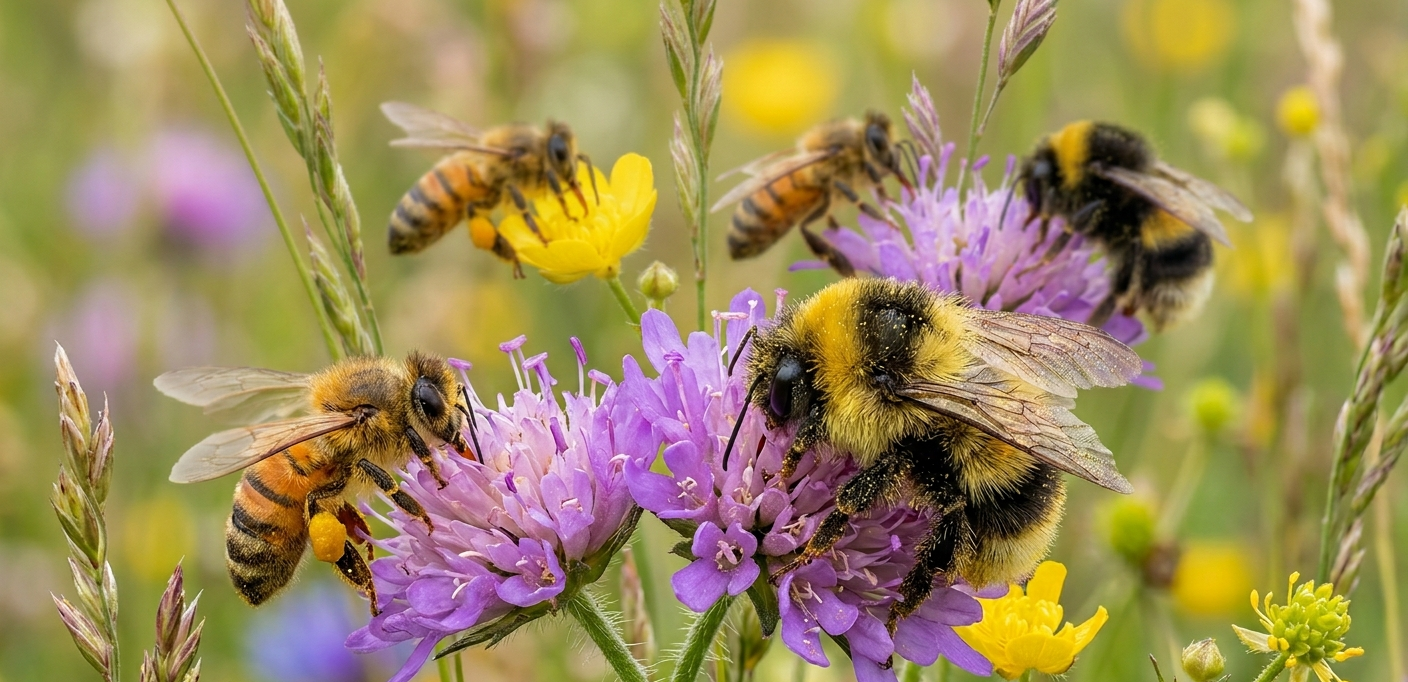
\includegraphics[width=\linewidth]{Figuras/Base_VC.png}
    \end{minipage}
    
    &
    % =========================
    % COLUMNA DERECHA (GRID 2x2)
    % =========================
    \begin{minipage}{0.48\textwidth}
        \centering
    
        \begin{tabular}{cc}
            \begin{minipage}{0.48\textwidth}
                \centering
                \textit{Volteo horizontal} \\[0.2cm]
                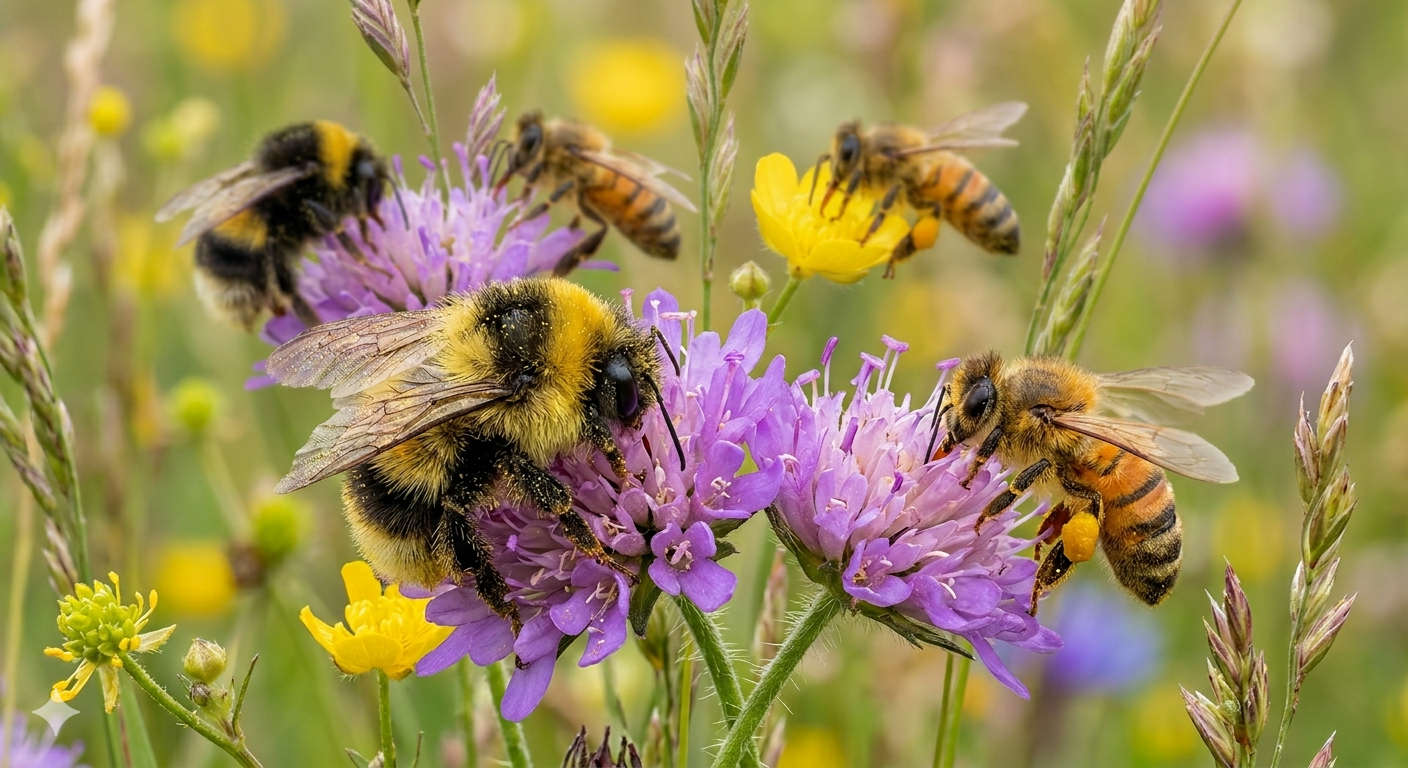
\includegraphics[width=\linewidth]{Figuras/flip.png}
            \end{minipage}
            &
            \begin{minipage}{0.48\textwidth}
                \centering
                \textit{Rotación} \\[0.2cm]
                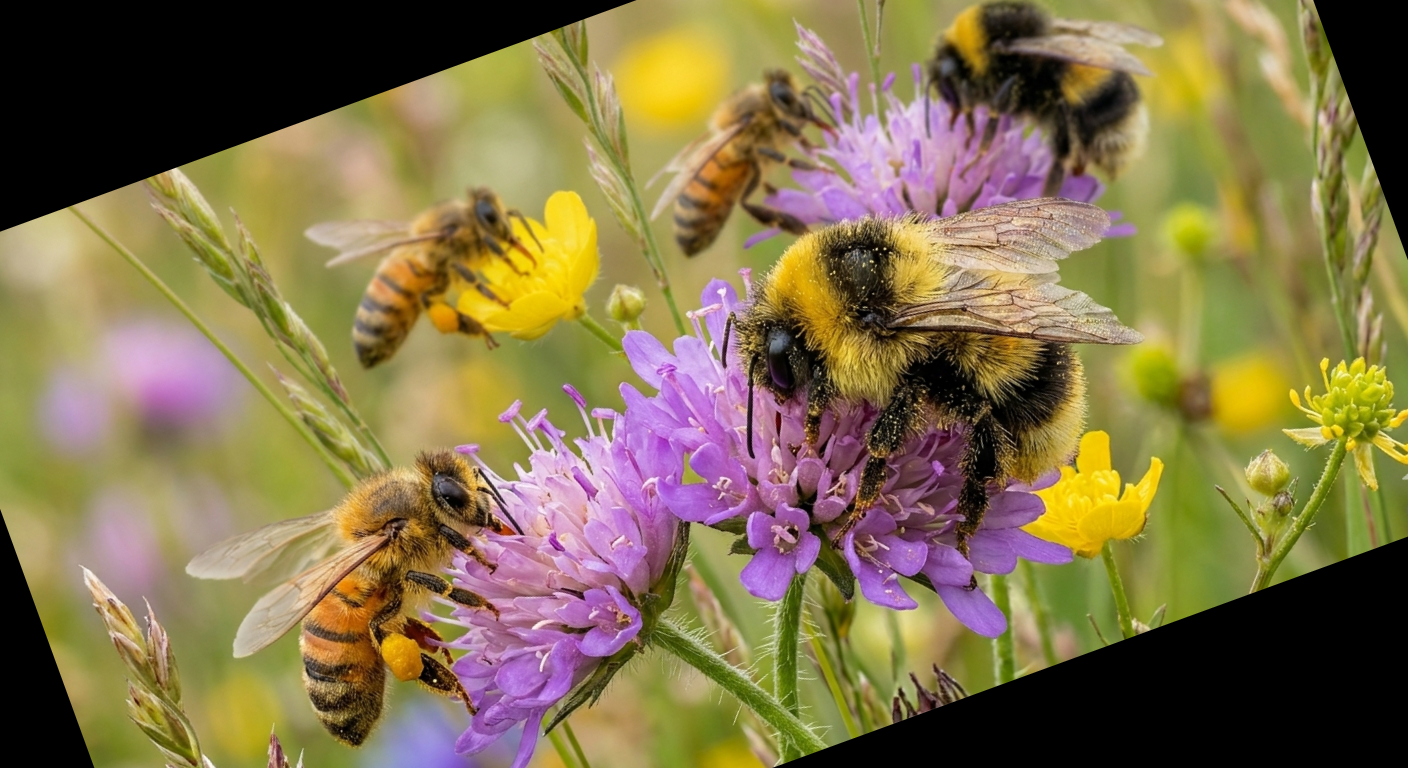
\includegraphics[width=\linewidth]{Figuras/rotacion.png}
            \end{minipage}
    
            \\[1.3 cm]
    
            \begin{minipage}{0.48\textwidth}
                \centering
                \textit{Escalamiento} \\[0.2cm]
                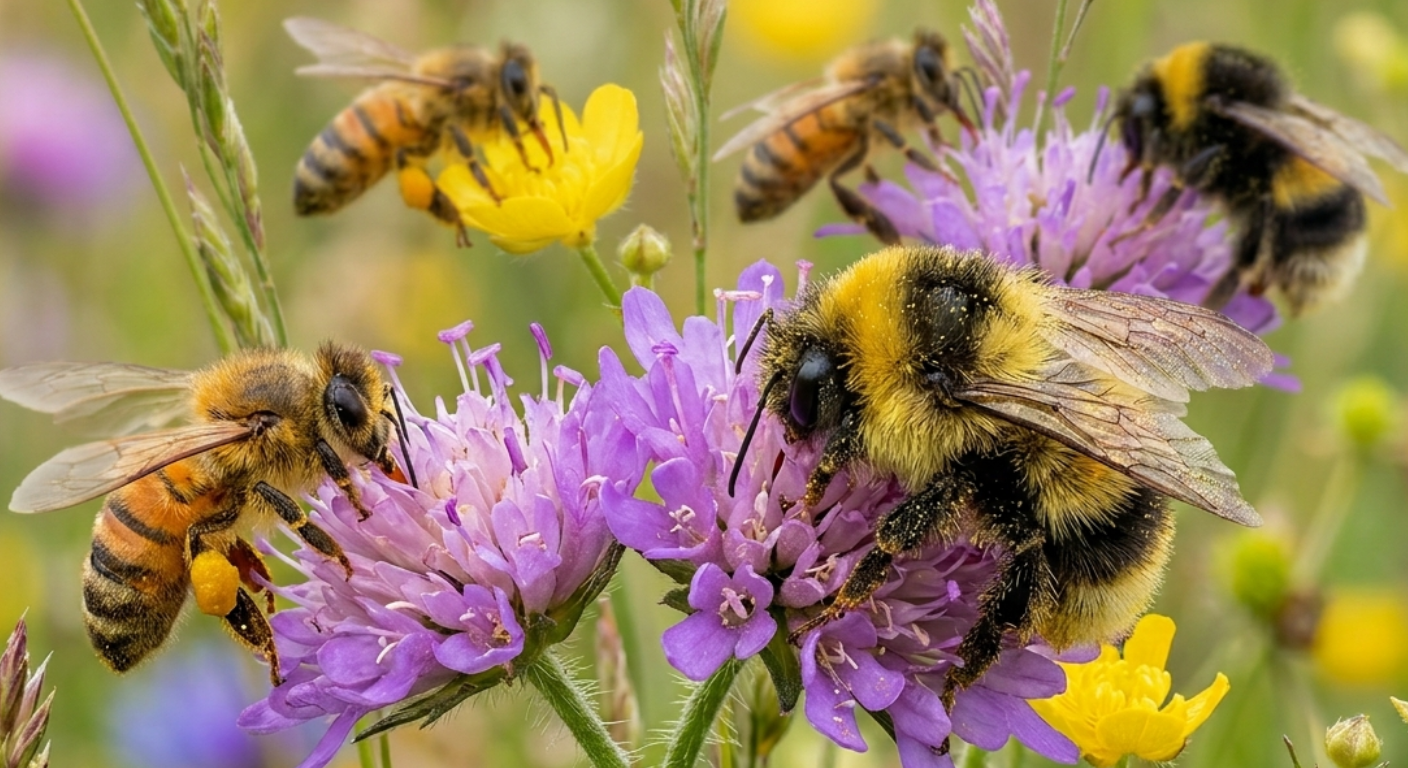
\includegraphics[width=\linewidth]{Figuras/scale.png}
            \end{minipage}
            &
            \begin{minipage}{0.48\textwidth}
                \centering
                \textit{Recorte} \\[0.2cm]
                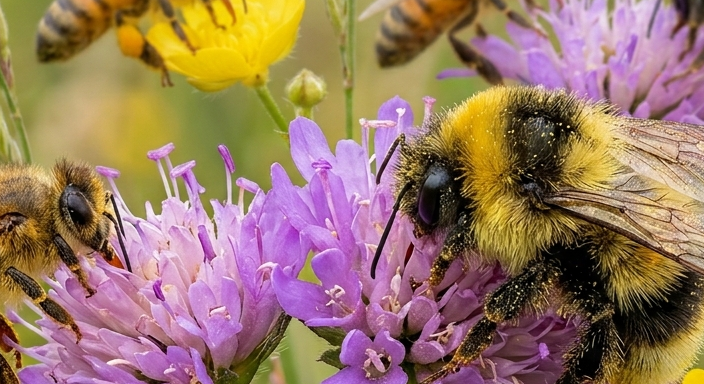
\includegraphics[width=\linewidth]{Figuras/crop.png}
            \end{minipage}
        \end{tabular}
    
    \end{minipage}
    
    \end{tabular}
    
    \label{fig:geom_transformations}

    \vspace{0.2cm}
    
    \caption*{\normalfont\normalsize\textit{Nota.} Elaboración propia.}
    
\end{figure}

\vspace{-1.0cm}

\subsubsection{Transformaciones fotométricas}

Las transformaciones fotométricas modifican brillo (\textit{brightness}), contraste (\textit{contrast}) y variaciones de color (\textit{color jitter}). Su objetivo es disminuir la sensibilidad del modelo a cambios de iluminación en entornos naturales \parencite{Kaur2022,Qian2023,Agarwal2025}. En la Figura \ref{fig:photometric_transformations} se indica un ejemplo con las distintas transformaciones. \\

\begin{figure}[H]
    \centering
    \caption{Ejemplo de transformaciones fotométricas.}
    
    \setlength{\tabcolsep}{6pt}
    
    \begin{tabular}{cc}
    
    % =========================
    % COLUMNA IZQUIERDA (ORIGINAL)
    % =========================
    \begin{minipage}{0.48\textwidth}
        \centering
        \textit{Imagen original} \\[0.25cm]
        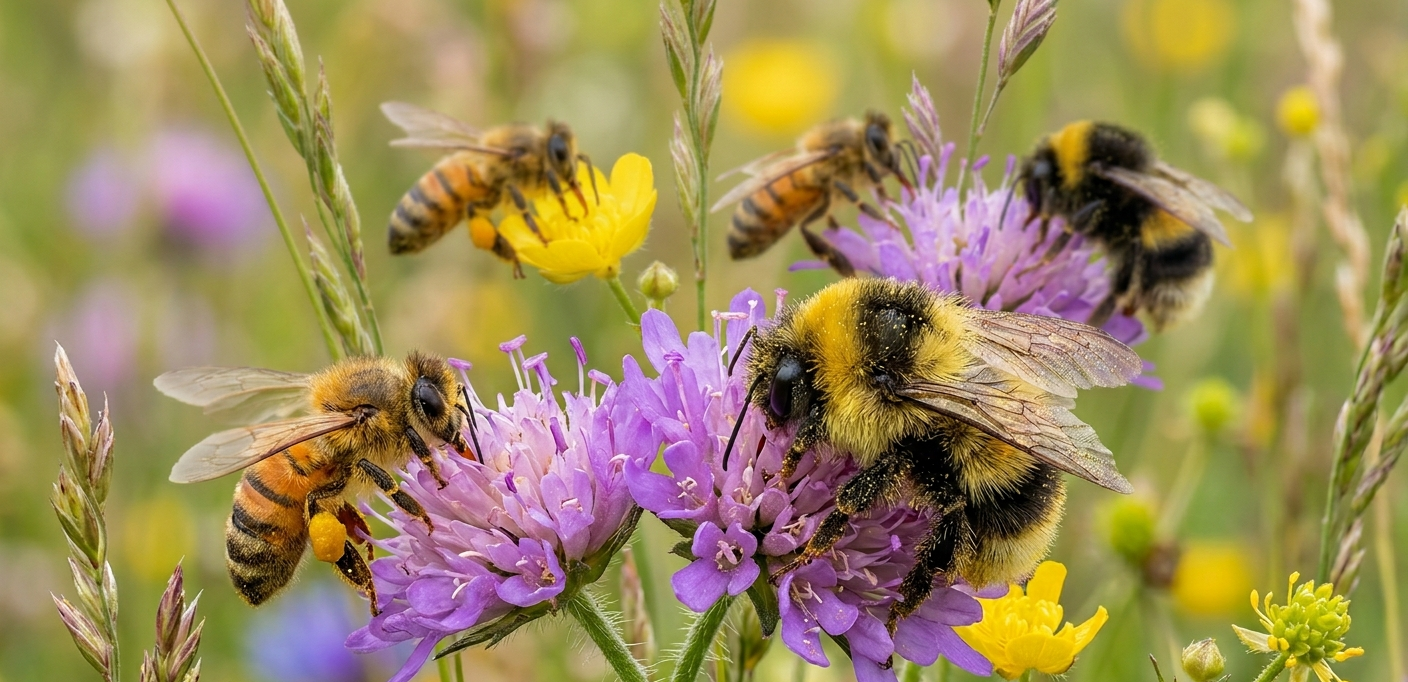
\includegraphics[width=\linewidth]{Figuras/Base_VC.png}
    \end{minipage}
    
    &
    % =========================
    % COLUMNA DERECHA (GRID 2x2)
    % =========================
    \begin{minipage}{0.48\textwidth}
        \centering
    
        \begin{tabular}{cc}
            \begin{minipage}{0.48\textwidth}
                \centering
                \textit{Brillo} \\[0.25cm]
                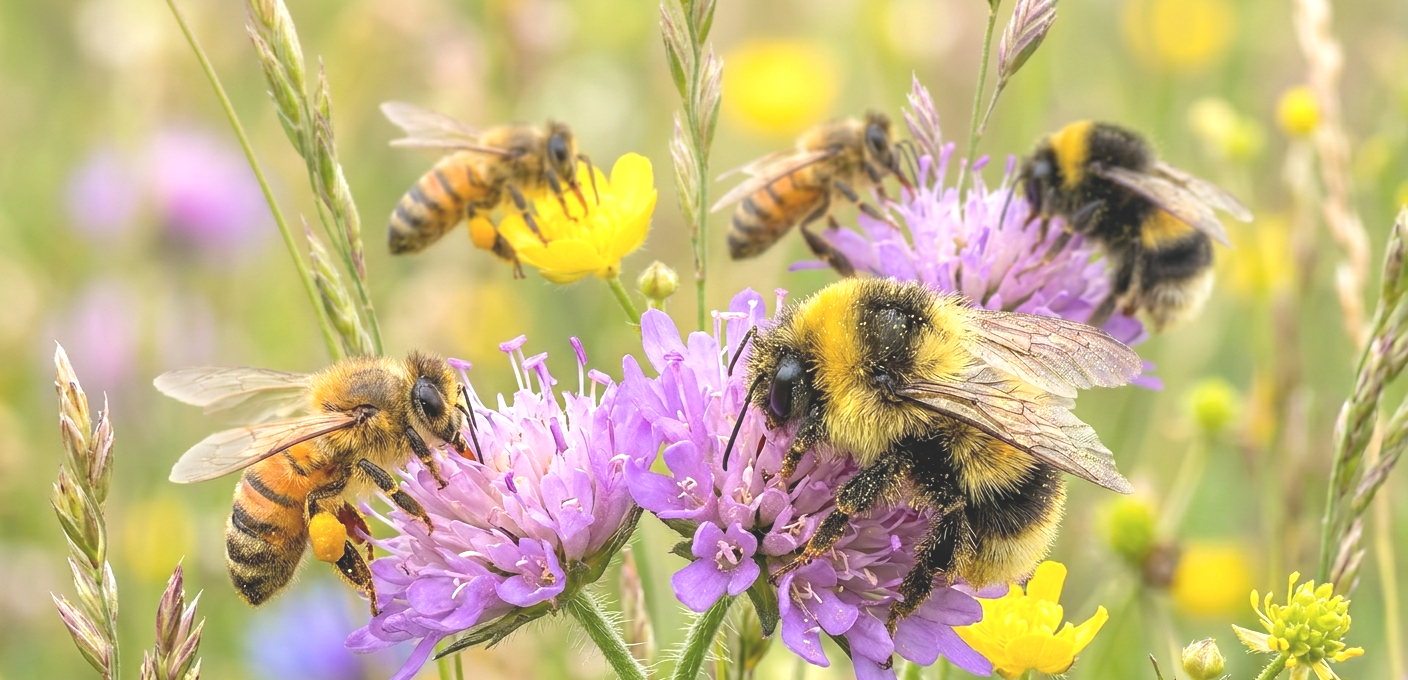
\includegraphics[width=\linewidth]{Figuras/brightness.png}
            \end{minipage}
            &
            \begin{minipage}{0.48\textwidth}
                \centering
                \textit{Contraste} \\[0.25cm]
                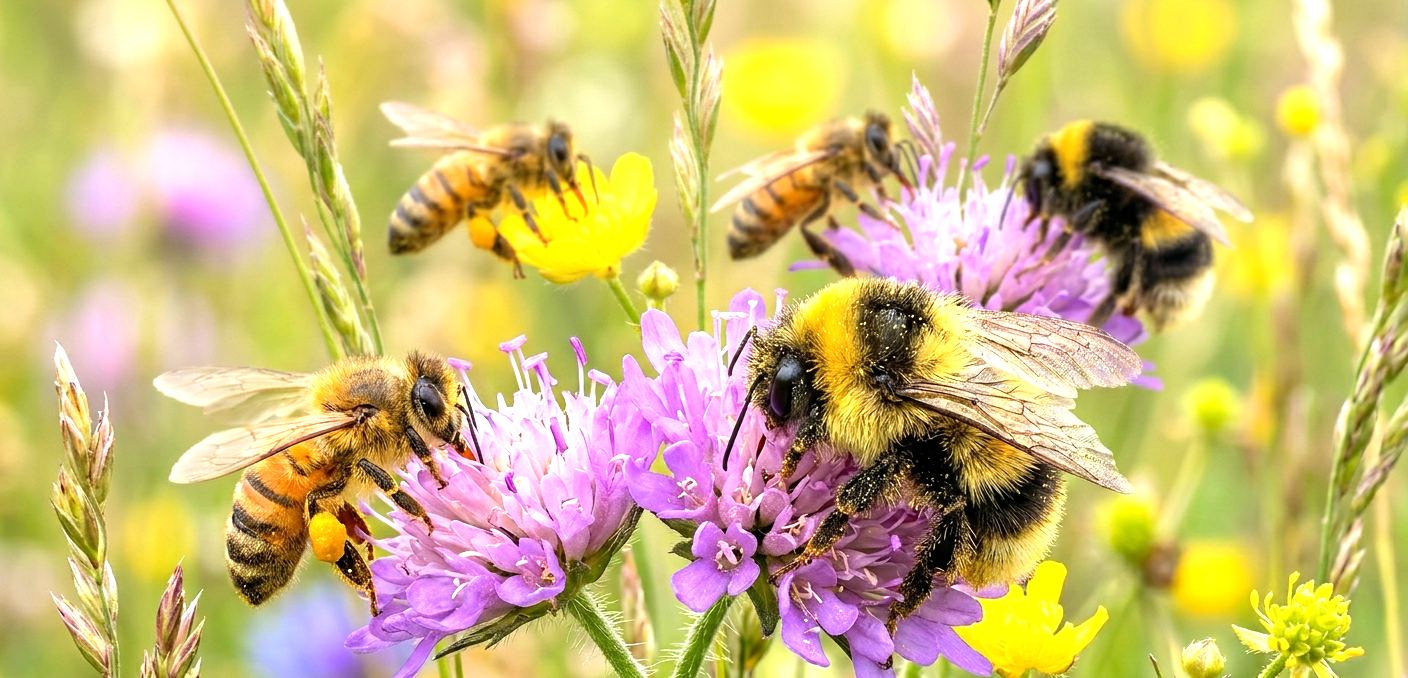
\includegraphics[width=\linewidth]{Figuras/contrast.png}
            \end{minipage}
    
            \\[1.2 cm]
    
            \begin{minipage}{0.48\textwidth}
                \centering
                \textit{Brillo + contraste} \\[0.25cm]
                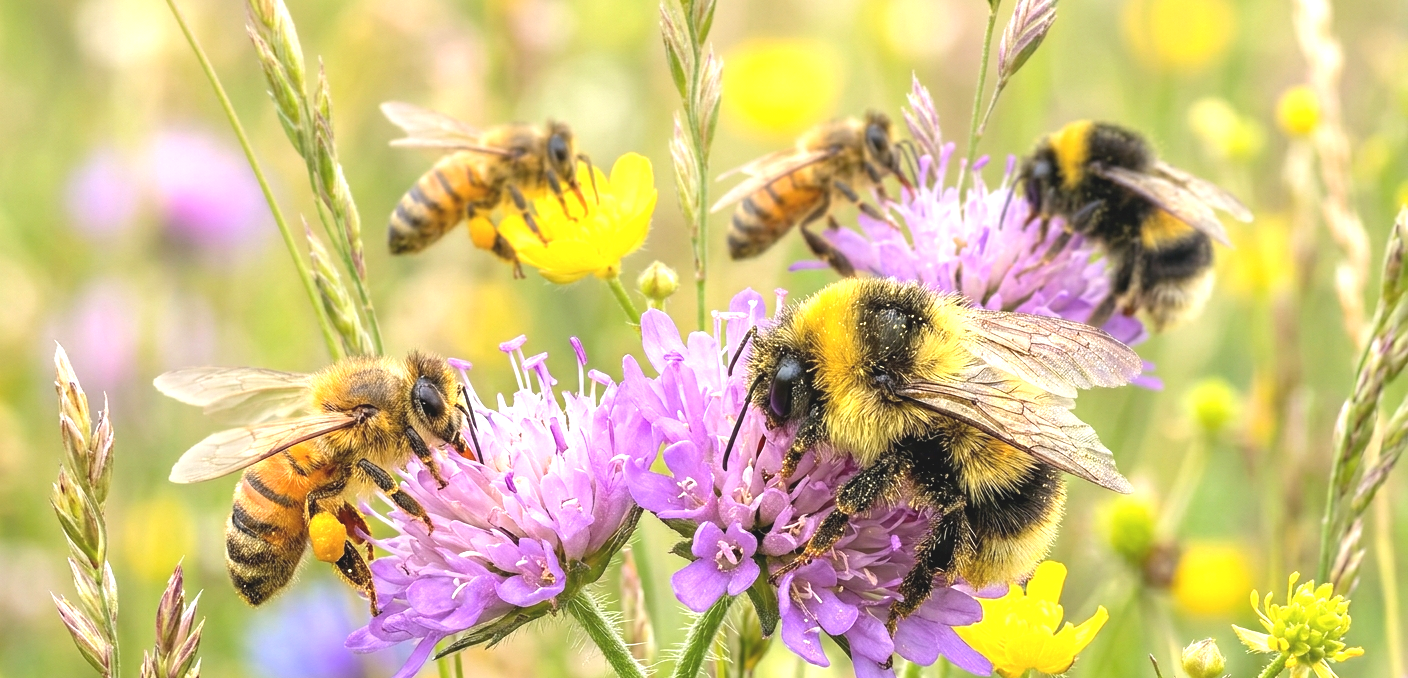
\includegraphics[width=\linewidth]{Figuras/brightness_contrast.png}
            \end{minipage}
            &
            \begin{minipage}{0.48\textwidth}
                \centering
                \textit{Variaciones de color} \\[0.25cm]
                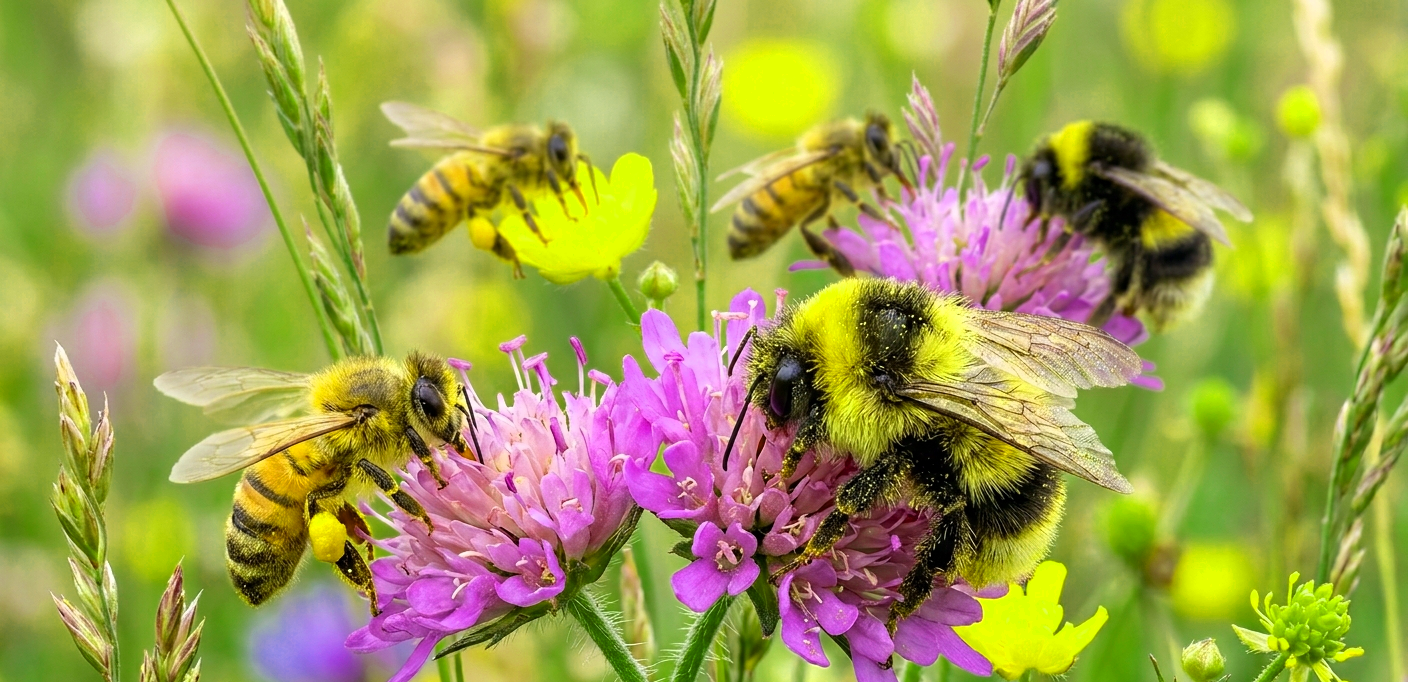
\includegraphics[width=\linewidth]{Figuras/color_jitter.png}
            \end{minipage}
        \end{tabular}
    
    \end{minipage}
    
    \end{tabular}
    
    \label{fig:photometric_transformations}
    
    \vspace{0.2cm}
    
    \caption*{\normalfont\normalsize\textit{Nota.} Elaboración propia.}

\end{figure}

\subsubsection{Ruido y desenfoque}

La adición de ruido (\textit{noise}) y desenfoque (\textit{blur}) aproxima imperfecciones reales del sensor o movimiento, lo cual incrementa la tolerancia del modelo a imágenes degradadas \parencite{Andriyanov2020,Madaan2024,Agarwal2025}. En la Figura \ref{fig:noise_blur} se indica un ejemplo con este tipo de imperfecciones. \\ 

\begin{figure}[H]
    \centering
    \caption{Ejemplo de ruido y desenfoque.}
    
    \setlength{\tabcolsep}{6pt}
    
    \begin{tabular}{cc}
    
    % =========================
    % FILA 1
    % =========================
    \begin{minipage}{0.45\textwidth}
        \centering
        \textit{Imagen original} \\[0.3cm]
        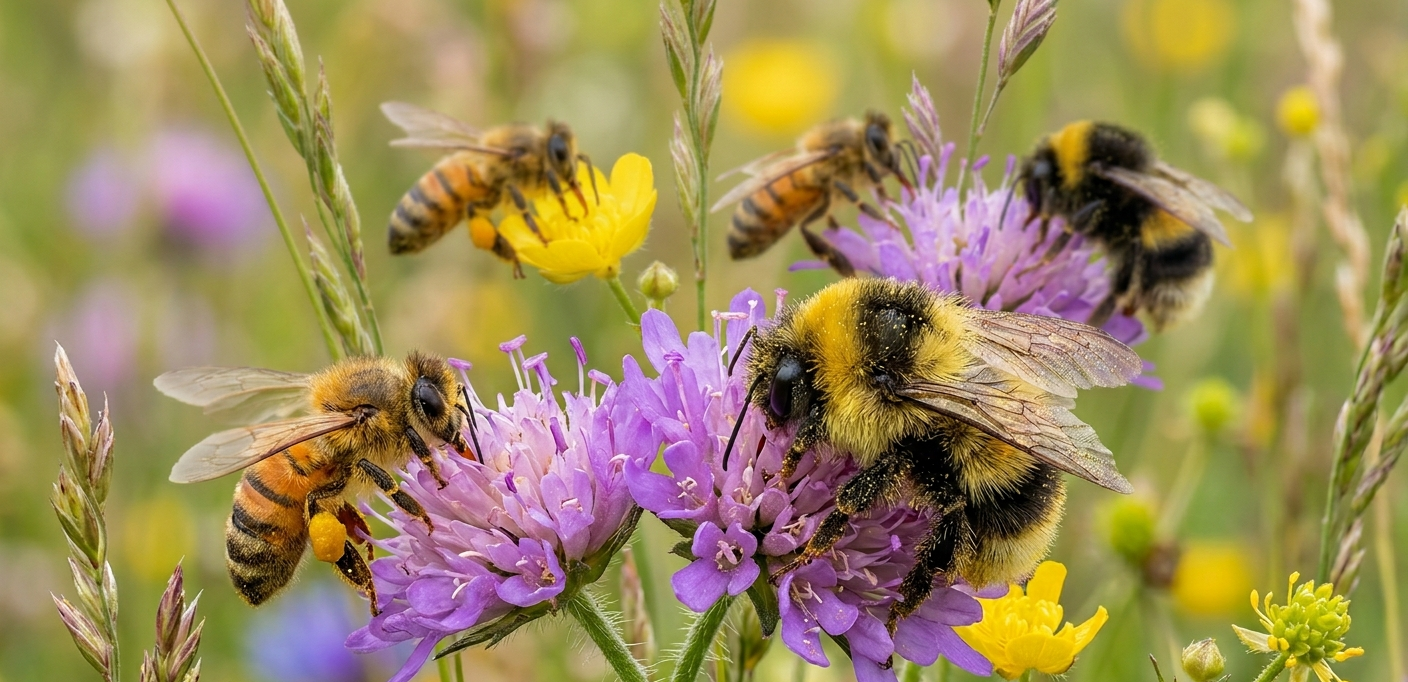
\includegraphics[width=\linewidth]{Figuras/Base_VC.png}
    \end{minipage}
    &
    \begin{minipage}{0.45\textwidth}
        \centering
        \textit{Ruido gaussiano} \\[0.3cm]
        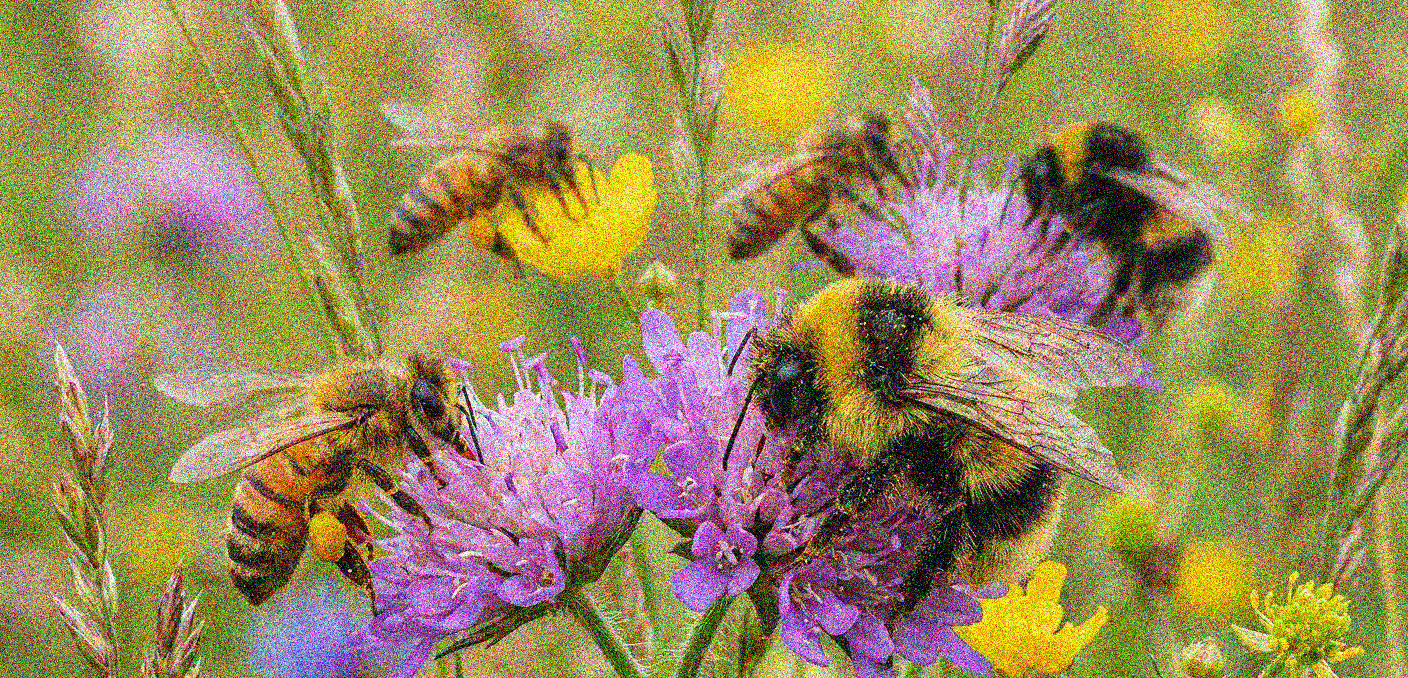
\includegraphics[width=\linewidth]{Figuras/gaussian_noise.png}
    \end{minipage}
    
    \\[2.0cm]
    
    % =========================
    % FILA 2
    % =========================
    \begin{minipage}{0.45\textwidth}
        \centering
        \textit{Desenfoque gaussiano} \\[0.3cm]
        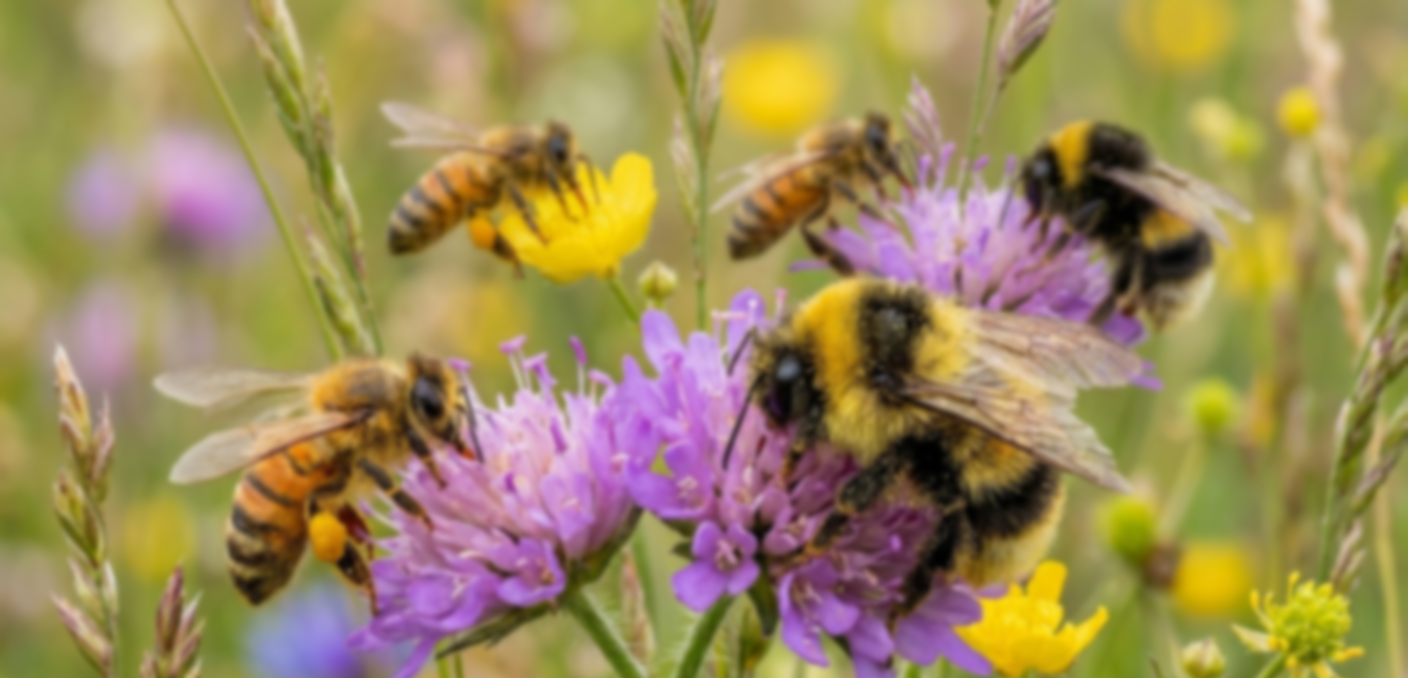
\includegraphics[width=\linewidth]{Figuras/gaussian_blur.png}
    \end{minipage}
    &
    \begin{minipage}{0.45\textwidth}
        \centering
        \textit{Desenfoque por movimiento} \\[0.3cm]
        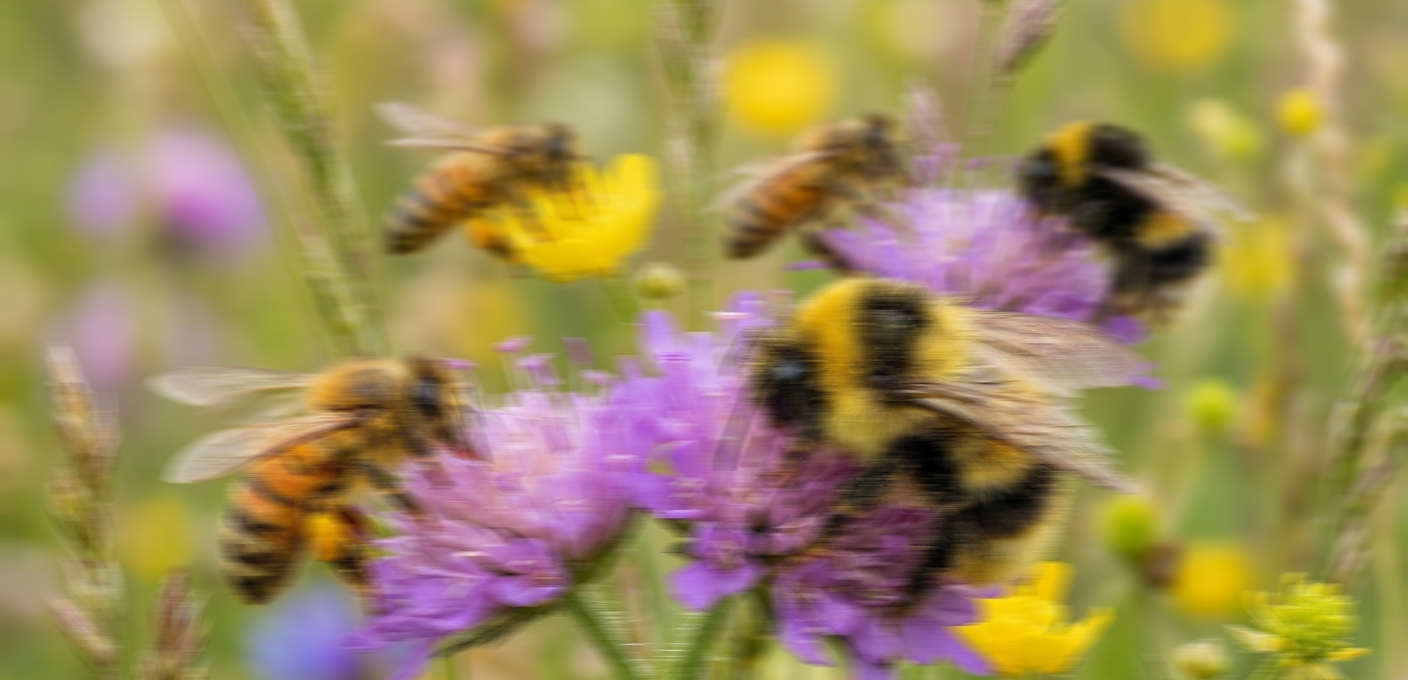
\includegraphics[width=\linewidth]{Figuras/motion_blur.png}
    \end{minipage}
    
    \end{tabular}
    
    \label{fig:noise_blur}
    \vspace{0.2cm}
    \caption*{\normalfont\normalsize\textit{Nota.} Elaboración propia.}

\end{figure}

\vspace{-1.0cm}
\subsubsection{Métodos avanzados y estrategias automáticas}

Métodos como MixUp, CutMix y Mosaic combinan muestras para aumentar la diversidad del conjunto de entrenamiento y reducir el sobreajuste, tal como se indica en la Figura \ref{fig:advanced_transformations}. Además, las estrategias automáticas de aumento de datos permiten seleccionar o aprender automáticamente combinaciones de transformaciones, como recorte, rotación, cambio de escala, brillo o contraste, de acuerdo con la tarea y las características del conjunto de datos. A diferencia de una política manual fija, estas estrategias buscan optimizar qué transformaciones aplicar y con qué intensidad para mejorar la generalización del modelo, especialmente en tareas de detección \parencite{Agarwal2025,Qian2023}. \\

\begin{figure}[H]
    \centering
    \caption{Ejemplo de técnicas avanzadas de aumento de datos.}
    
    \setlength{\tabcolsep}{6pt}
    
    % =========================
    % FILA SUPERIOR (IMÁGENES BASE)
    % =========================
    \begin{tabular}{cc}
    
    \begin{minipage}{0.45\textwidth}
        \centering
        \textit{Imagen original 1} \\[0.3cm]
        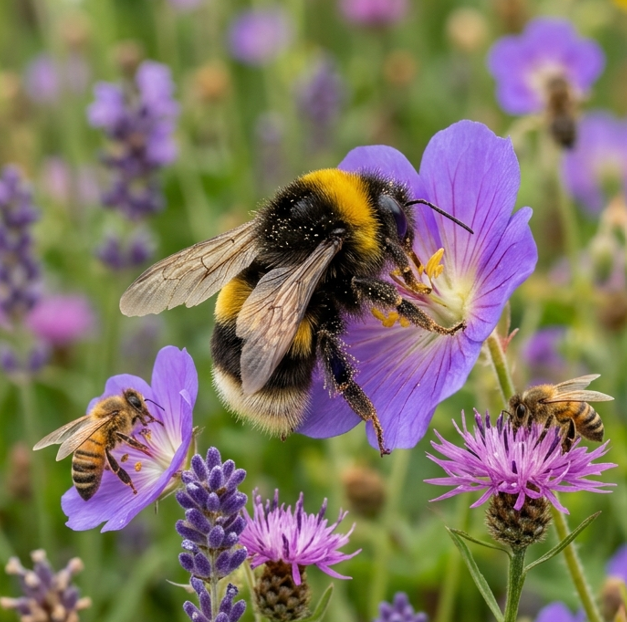
\includegraphics[width=6cm, height=3.5 cm]{Figuras/Base_DA_01.png}
    \end{minipage}
    &
    \begin{minipage}{0.45\textwidth}
        \centering
        \textit{Imagen original 2} \\[0.3cm]
        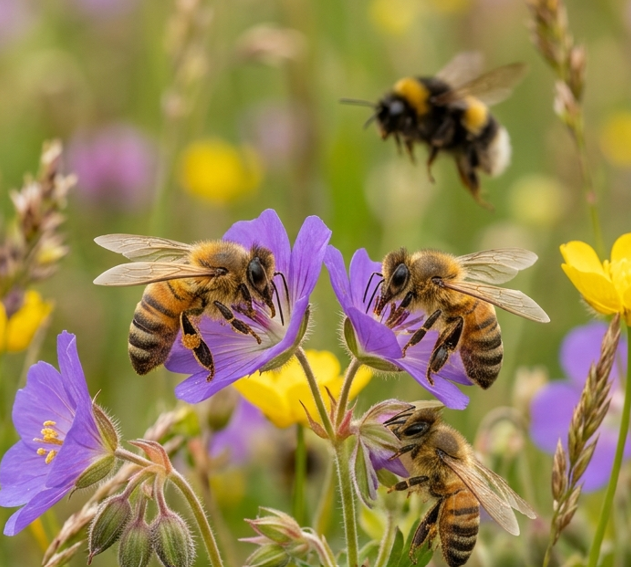
\includegraphics[width=6cm, height=3.5cm]{Figuras/Base_DA_02.png}
    \end{minipage}
    
    \end{tabular}
    
    \vspace{0.6cm}
    
    % =========================
    % FILA INFERIOR (MÉTODOS)
    % =========================
    \begin{tabular}{ccc}
    
    \begin{minipage}{0.3\textwidth}
        \centering
        \textit{MixUp} \\[0.25cm]
        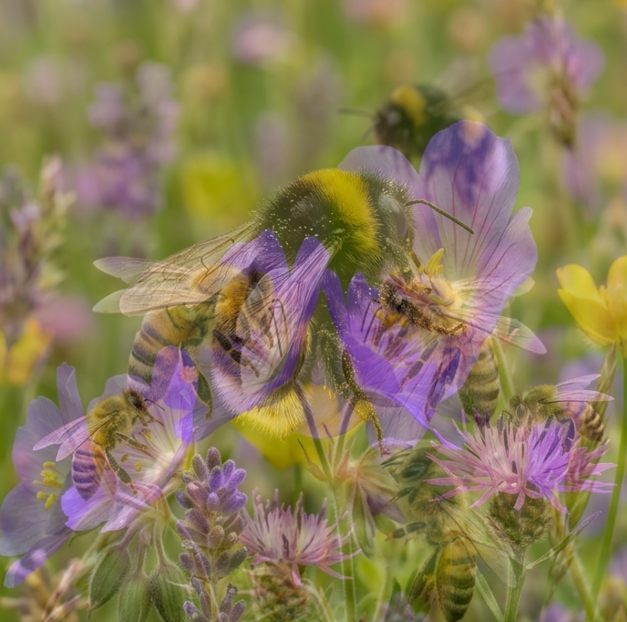
\includegraphics[width=5 cm,height=3.5cm]{Figuras/mixup.png}
    \end{minipage}
    &
    \begin{minipage}{0.3\textwidth}
        \centering
        \textit{CutMix} \\[0.25cm]
        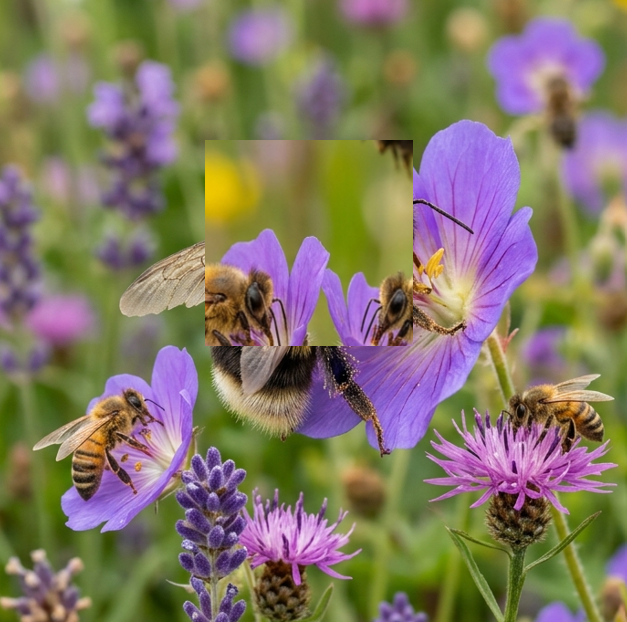
\includegraphics[width=5 cm, height=3.5cm]{Figuras/cutmix.png}
    \end{minipage}
    &
    \begin{minipage}{0.3\textwidth}
        \centering
        \textit{Mosaic} \\[0.25cm]
        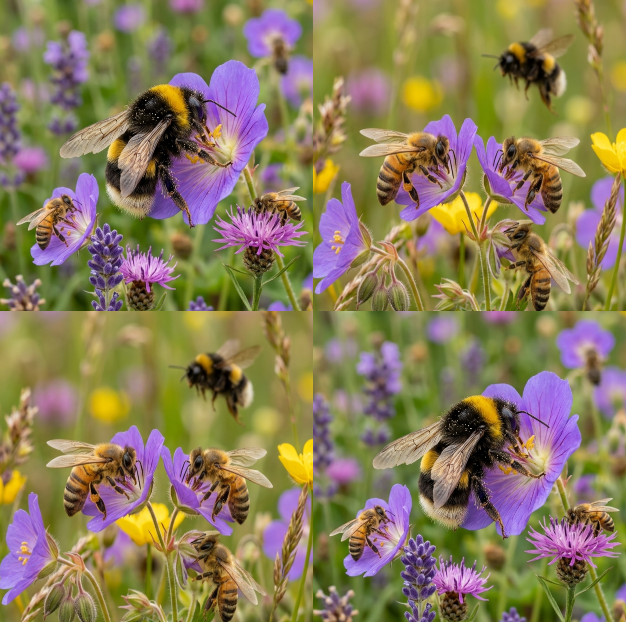
\includegraphics[width=5 cm, height=3.5cm]{Figuras/mosaic.png}
    \end{minipage}
    
    \end{tabular}
    
    \label{fig:advanced_transformations}

    \vspace{0.2cm}
    \caption*{\normalfont\normalsize\textit{Nota.} Elaboración propia.}
\end{figure}

\vspace{-1.0cm}
\subsubsection{Segmentación y aumento basado en objetos}

En segmentación, el aumento basado en objetos inserta o compone instancias para reforzar el aprendizaje de bordes y regiones, siendo útil cuando la clase objetivo ocupa un área pequeña o existe alta variabilidad de fondo \parencite{Illarionova2021,Chen2024}. En la Figura \ref{fig:object_based_augmentation} se indica un ejemplo con estas variaciones. \\

\begin{figure}[H]
\centering
\caption{Ejemplo de segmentación y aumento basado en objetos.}

\setlength{\tabcolsep}{8pt}

\begin{tabular}{cc}

\begin{minipage}{0.45\textwidth}
    \centering
    \textit{Imagen original} \\[0.3cm]
    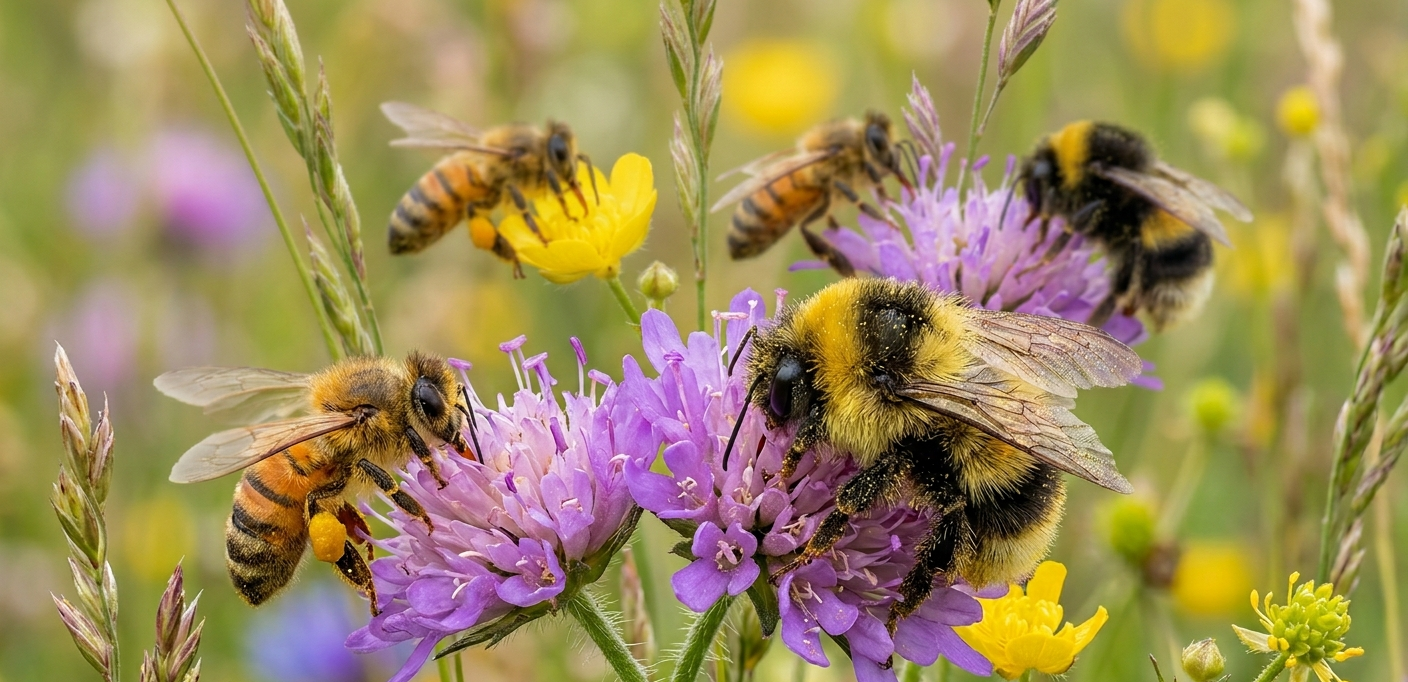
\includegraphics[width=0.9\linewidth, keepaspectratio]{Figuras/Base_VC.png}
\end{minipage}
&
\begin{minipage}{0.45\textwidth}
    \centering
    \textit{Aumento basado en objetos} \\[0.3cm]
    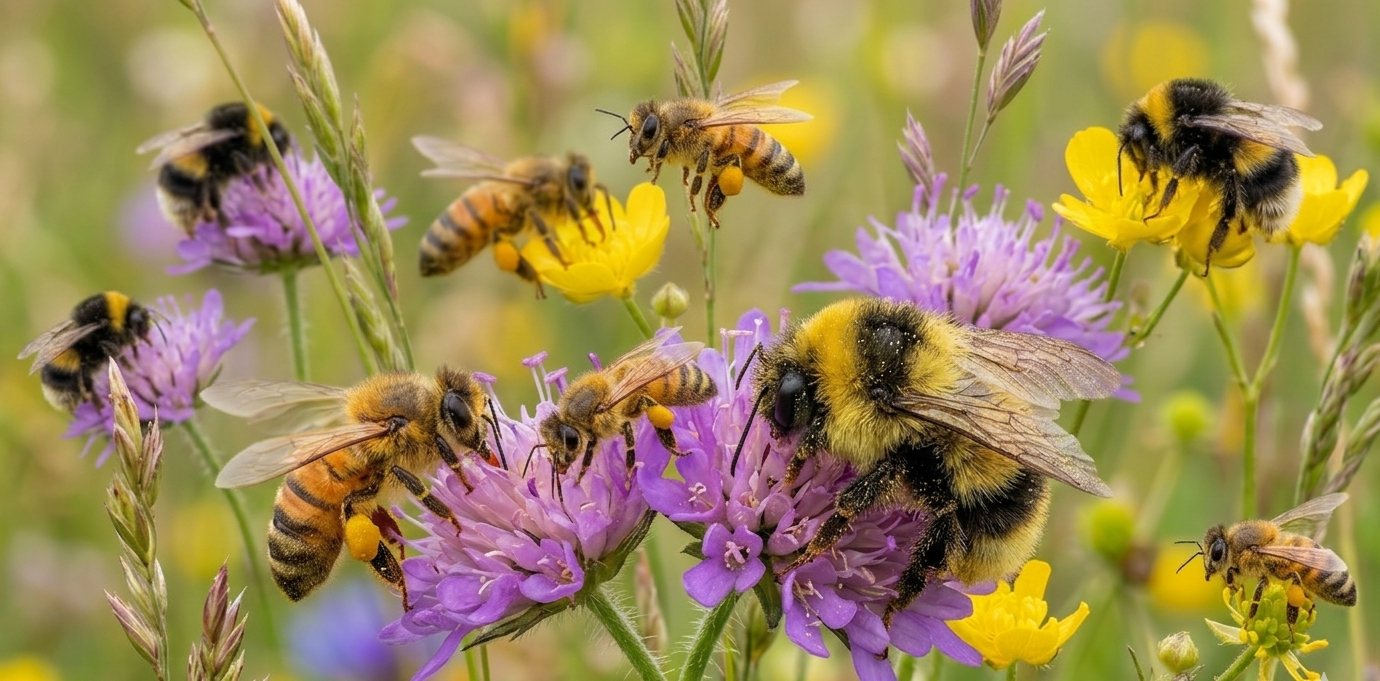
\includegraphics[width=0.9\linewidth, keepaspectratio]{Figuras/Seg_aumento_datos.png}
\end{minipage}

\end{tabular}

\label{fig:object_based_augmentation}

\vspace{0.2cm}
\caption*{\normalfont\normalsize\textit{Nota.} Elaboración propia.}

\end{figure}

\vspace{-1.0cm}
\subsection{Métodos de optimización}

Los métodos de optimización, como el descenso de gradiente y sus variantes ajustan los parámetros de las redes neuronales para minimizar la función de pérdida \parencite{rudenko2020optimization}. En el reconocimiento de polinizadores, estos métodos son esenciales para un entrenamiento eficiente y para evitar el sobreajuste mediante técnicas como regularización y
abandono, garantizando un buen rendimiento con datos nuevos.

En esta sección se describen los principales métodos y estrategias asociados al entrenamiento de redes neuronales profundas. Además de los algoritmos de optimización propiamente dichos, como SGD, Adam, RMSProp y AdamW, se consideran estrategias complementarias que influyen en la estabilidad y generalización del modelo, tales como el muestreo estratificado, las políticas de tasa de aprendizaje, la regularización y la estabilidad. 

\par\indent\textbullet\hspace{0.2cm} \textbf{Descenso de Gradiente Estocástico:} también llamado SGD, es un referente por su comportamiento estable, aunque puede converger más lentamente; su variante con \textit{momentum} incorpora una acumulación de gradientes que acelera el avance en direcciones consistentes \parencite{Postalcloǧlu2020,Sudewo2025}. 

\par\indent\textbullet\hspace{0.2cm} \textbf{Optimizadores adaptativos:} ajustan tasas de aprendizaje por parámetro y suelen mejorar la rapidez de convergencia; sin embargo, su desempeño final depende del dominio y de la configuración de hiperparámetros \parencite{Postalcloǧlu2020,Azis2025}. RMSProp adapta la tasa de aprendizaje mediante un promedio móvil de los gradientes cuadrados, lo que ayuda a estabilizar el entrenamiento cuando existen variaciones fuertes en los gradientes. Adam combina esta adaptación con el uso de momentos del gradiente, mientras que AdamW desacopla el \textit{weight decay} de la actualización del gradiente, lo que puede favorecer la generalización frente a Adam en prácticas modernas de entrenamiento \parencite{Azis2025,Sudewo2025}.

\par\indent\textbullet\hspace{0.2cm} \textbf{Optimizadores recientes y enfoques híbridos:} métodos como DiffGrad y AdaNorm introducen correcciones dinámicas basadas en el comportamiento o norma del gradiente para estabilizar el entrenamiento y mejorar el ajuste en CNN \parencite{Dubey2020,Dubey2023}. En paralelo, enfoques híbridos exploran combinar optimizadores adaptativos y tradicionales para conservar convergencia rápida sin degradar la generalización \parencite{Pattanaik2025}. 

\par\indent\textbullet\hspace{0.2cm} \textbf{Muestreo estratificado:} es una técnica que divide la población en subgrupos para mantener proporciones representativas y evitar sesgos por desbalance. En estudios de polinizadores, permite incluir adecuadamente clases raras como parásitos o anomalías, mejorando el aprendizaje del modelo y su capacidad de generalizar en distintos entornos \parencite{lee2025enhancing}

\par\indent\textbullet\hspace{0.2cm} \textbf{Políticas de tasa de aprendizaje:} regulan $\eta_t$ durante el entrenamiento. Esquemas como \textit{step decay}, \textit{cosine annealing} y \textit{warmup} pueden mejorar la convergencia y evitar estancamiento en tareas de clasificación visual \parencite{Xue2022}.

\par\indent\textbullet\hspace{0.2cm} \textbf{Regularización y estabilidad:} el \textit{weight decay} controla el crecimiento de pesos y contribuye a la generalización, mientras que \textit{early stopping} detiene el entrenamiento cuando la validación deja de mejorar, reduciendo sobreajuste y costo computacional \parencite{Azis2025,Loganathan2025}. El \textit{gradient clipping} limita $\|\nabla_{\theta}\mathcal{L}\|$ para evitar explosiones de gradiente en entrenamientos inestables \parencite{Xue2022}.
